\section{Disordered Kagome lattice with emergent holographic physics}
\subsection{Fermionic flatband systems and complex SYK model}
%----------------------------------------------------------------------------------------
\begin{frame}{Flat band systems}

\begin{block}{Flat band systems}
Flatband systems are systems whose kinetic energy are independent or weakly-dependent on (quasi-)momentum i.e., $\nabla_{\mathbf{k}} E(\mathbf{k}) \approx 0$
\end{block}

\begin{block}{Examples}
    Fermions in kagome lattice, magic angle twisted bilayer graphene, ...
\end{block}

\end{frame}
%----------------------------------------------------------------------------------------
\begin{frame}{Quantum chaos}

\begin{figure}
    \centering
    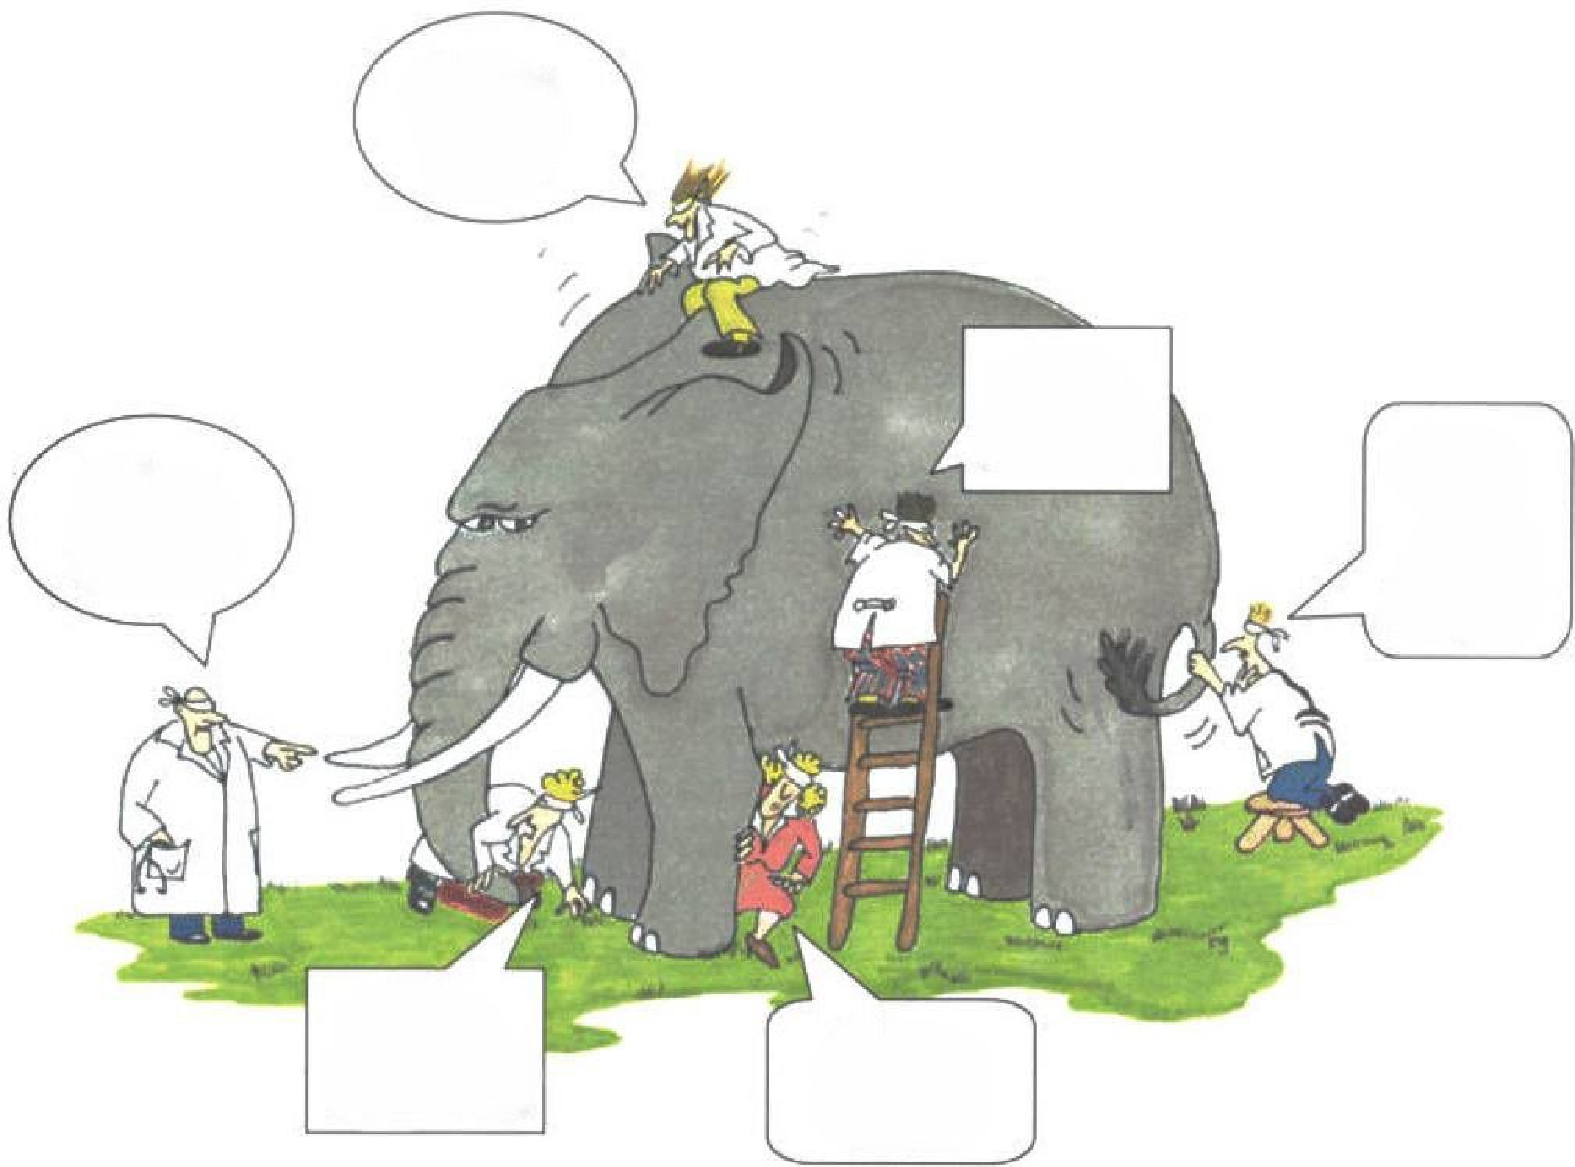
\includegraphics[width=0.6\linewidth]{figs/bme.pdf}
    \begin{picture}(0,0)
    {\def\unitlength{}
    \put(-0.36\linewidth,0.28\linewidth){\text{\color{white} \tiny Quantum chaos}}
    %
    \put(-0.59\linewidth,0.245\linewidth){\text{\tiny Wigner Dyson}}
    \put(-0.58\linewidth,0.235\linewidth){\text{\tiny ensemble}}
    %
    \put(-0.44\linewidth,0.41\linewidth){\text{\tiny out-of-}}
    \put(-0.46\linewidth,0.40\linewidth){\text{\tiny time-ordered}}
    \put(-0.45\linewidth,0.39\linewidth){\text{\tiny correlator}}
    %
    \put(-0.31\linewidth,0.04\linewidth){\text{\tiny quantum}}
    \put(-0.31\linewidth,0.03\linewidth){\text{\tiny computational}}
    \put(-0.31\linewidth,0.02\linewidth){\text{\tiny complexity}}
    %
    \put(-0.48\linewidth,0.04\linewidth){\text{\tiny Krylov}}
    \put(-0.48\linewidth,0.03\linewidth){\text{\tiny complexity}}
    %
    \put(-0.23\linewidth,0.285\linewidth){\text{\tiny $k$-design}}
    %
    \put(-0.06\linewidth,0.24\linewidth){\text{\tiny $\cdots$}}
    }
    \end{picture}
\end{figure}

\end{frame}
%----------------------------------------------------------------------------------------
\begin{frame}{Complex SYK model}

\begin{block}{}
\begin{equation*}
    \mathcal{H}_{\mathrm{SYK}} = -\mu\sum_{i} c_{i}^{\dagger} c_{i} + \sum_{i>j,k>l}J_{ijkl} c_{i}^{\dagger} c_{j}^{\dagger} c_{k} c_{l}
    \quad
    \left\langle J_{ijkl} \right\rangle = 0
    ~
    \left\langle |J_{ijkl}|^2 \right\rangle = \frac{J^2}{2N^3}
\end{equation*}

\begin{equation*}
    G(i\omega_n) = \frac{1}{i\omega_n + \mu - \Sigma(i\omega_n)}
    \quad
    \Sigma(\tau)
    =
    \vcenter{\hbox{
            \feynmandiagram [horizontal=f2 to f3] {
            f1 --  f2 -- f3 -- f4,
            f3 -- [bend left=30] f2,
            f3 -- [bend right=30] f2,
            f3 -- [scalar,bend right=80] f2,
            };}}
            = -J^2 G^2(\tau) G(-\tau)
\end{equation*}
\end{block}

At $N \gg 1$, $J\tau \gg 1$ and $\beta J \gg 1$\footnote[frame]{\cite{sachdev1993gapless,davison2017thermoelectric}}:
\begin{itemize}
\item Conformal invariance:
$\tau \to f(\tau),
G(\tau_1,\tau_2) \to f^{\prime}\left(\tau_{1}\right)^{\Delta} f^{\prime}\left(\tau_{2}\right)^{\Delta} e^{i\left(\phi\left(\tau_{1}\right)-\phi\left(\tau_{2}\right)\right)} G\left(f\left(\tau_{1}\right), f\left(\tau_{2}\right)\right)$

% \item Non-Fermi liquid: $G(\tau)=\frac{b}{\sqrt{|\tau|}}\operatorname{sgn}(\tau)$

\item Non-Fermi liquid:
%$G(\omega) \sim \frac{1}{\sqrt{|\omega|}}\operatorname{sgn}(\omega)$
$G(z) = C\frac{e^{-i(\pi/4 + \theta)}}{\sqrt{z}}$

\item $\rho(E) = -\frac{1}{\pi} \Im G(w+i0^{+}) \approx \sqrt{\left(1-E / E_{0}\right)}$

% \item AdS/CFT: $\begin{cases}
% S \sim - \int dt \{ f(t), t) \}
%         = - \int dt [ (\frac{f''}{f'})' - \frac{1}{2} \frac{f''^2}{f'^2} ] \\
% -\beta F_{\mathrm{JT}} = s_{0,\mathrm{JT}} + \frac{\pi \bar{\phi}}{4G \beta}
% \Longleftrightarrow
% -\beta F_{\mathrm{SYK}} = s_{0,\mathrm{SYK}} + \frac{c}{2 \beta}
% \end{cases}$

\item Chaotic out-of-time-ordered correlator(OTOC): $\frac{1}{N} \sum_i \langle c_{i}^{\dagger}(\tau) c_{i}(0) c_{i}^{\dagger}(\tau) c_{i}(0) \rangle = f_{0} - \frac{f_1}{N} e^{\frac{2\pi}{\beta}\tau}$
\end{itemize}

\end{frame}
%----------------------------------------------------------------------------------------
% \begin{frame}{Quantum chaos}

% Classically, a dynamical system is chaotic if it, at a minimum, satisfies%\cite{glendinning1994stability,devaney2018introduction}
% \begin{itemize}
%     \item sensitive to initial conditions;
%     \item topological mixing.
% \end{itemize}

% The quantum counterpart of "topological mixing" is random matrices theory (via the Bohigas-Giannoni-Schmit (BGS) conjecture)

% The quantum counterpart of "sensitive to initial conditions" can be
% \begin{itemize}
%     \item out-of-time-order correlator ($OTOC$)
%     \item $k$-design
%     \item quantum computational complexity
%     \item Krylov complexity
% \end{itemize}

% \end{frame}
%----------------------------------------------------------------------------------------
\subsection{Kagome lattice}
%----------------------------------------------------------------------------------------
\begin{frame}{Kagome lattice}

\begin{equation*}
    H = \eqnmarkbox[NavyBlue]{hoppings}{H_{t}}
    + \eqnmarkbox[OliveGreen]{disorder}{H_{D}}
    + \eqnmarkbox[WildStrawberry]{interaction}{H_{I}}
\end{equation*}
\annotate[yshift=0.5em]{above,left}{hoppings}{fermionic \& flatband}
\annotate[yshift=0.5em]{above, right}{disorder}{disorder}
\annotate[yshift=0.5em]{above, right}{interaction}{repulsion}

\vspace{-4mm}
\begin{block}{}%{Tight binding Hamiltonian of polarized fermions}
\begin{equation*}
\begin{aligned}
\mathcal{H}_{t}=&-\mu\sum_{m}(a_{\mathbf{r}_{m}}^{(a)\dagger}a_{\mathbf{r}_{m}}^{(a)}+a_{\mathbf{r}_{m}}^{(b)\dagger}a_{\mathbf{r}_{m}}^{(b)}+a_{\mathbf{r}_{m}}^{(c)\dagger}a_{\mathbf{r}_{m}}^{(c)})\\
&-t\sum_{<m,n>}e^{i\varphi}(a_{\mathbf{r}_m}^{(b)\dagger}a_{\mathbf{r}_n}^{(a)}+a_{\mathbf{{r}_m}}^{(a)\dagger}a_{\mathbf{r}_n}^{(c)}+a_{\mathbf{{r}_m}}^{(c)\dagger}a_{\mathbf{{r}_n}}^{(b)})+h.c.
\end{aligned}
\end{equation*}
\end{block}
\vspace{-1mm}

\begin{figure}
\begin{minipage}{0.5\linewidth}
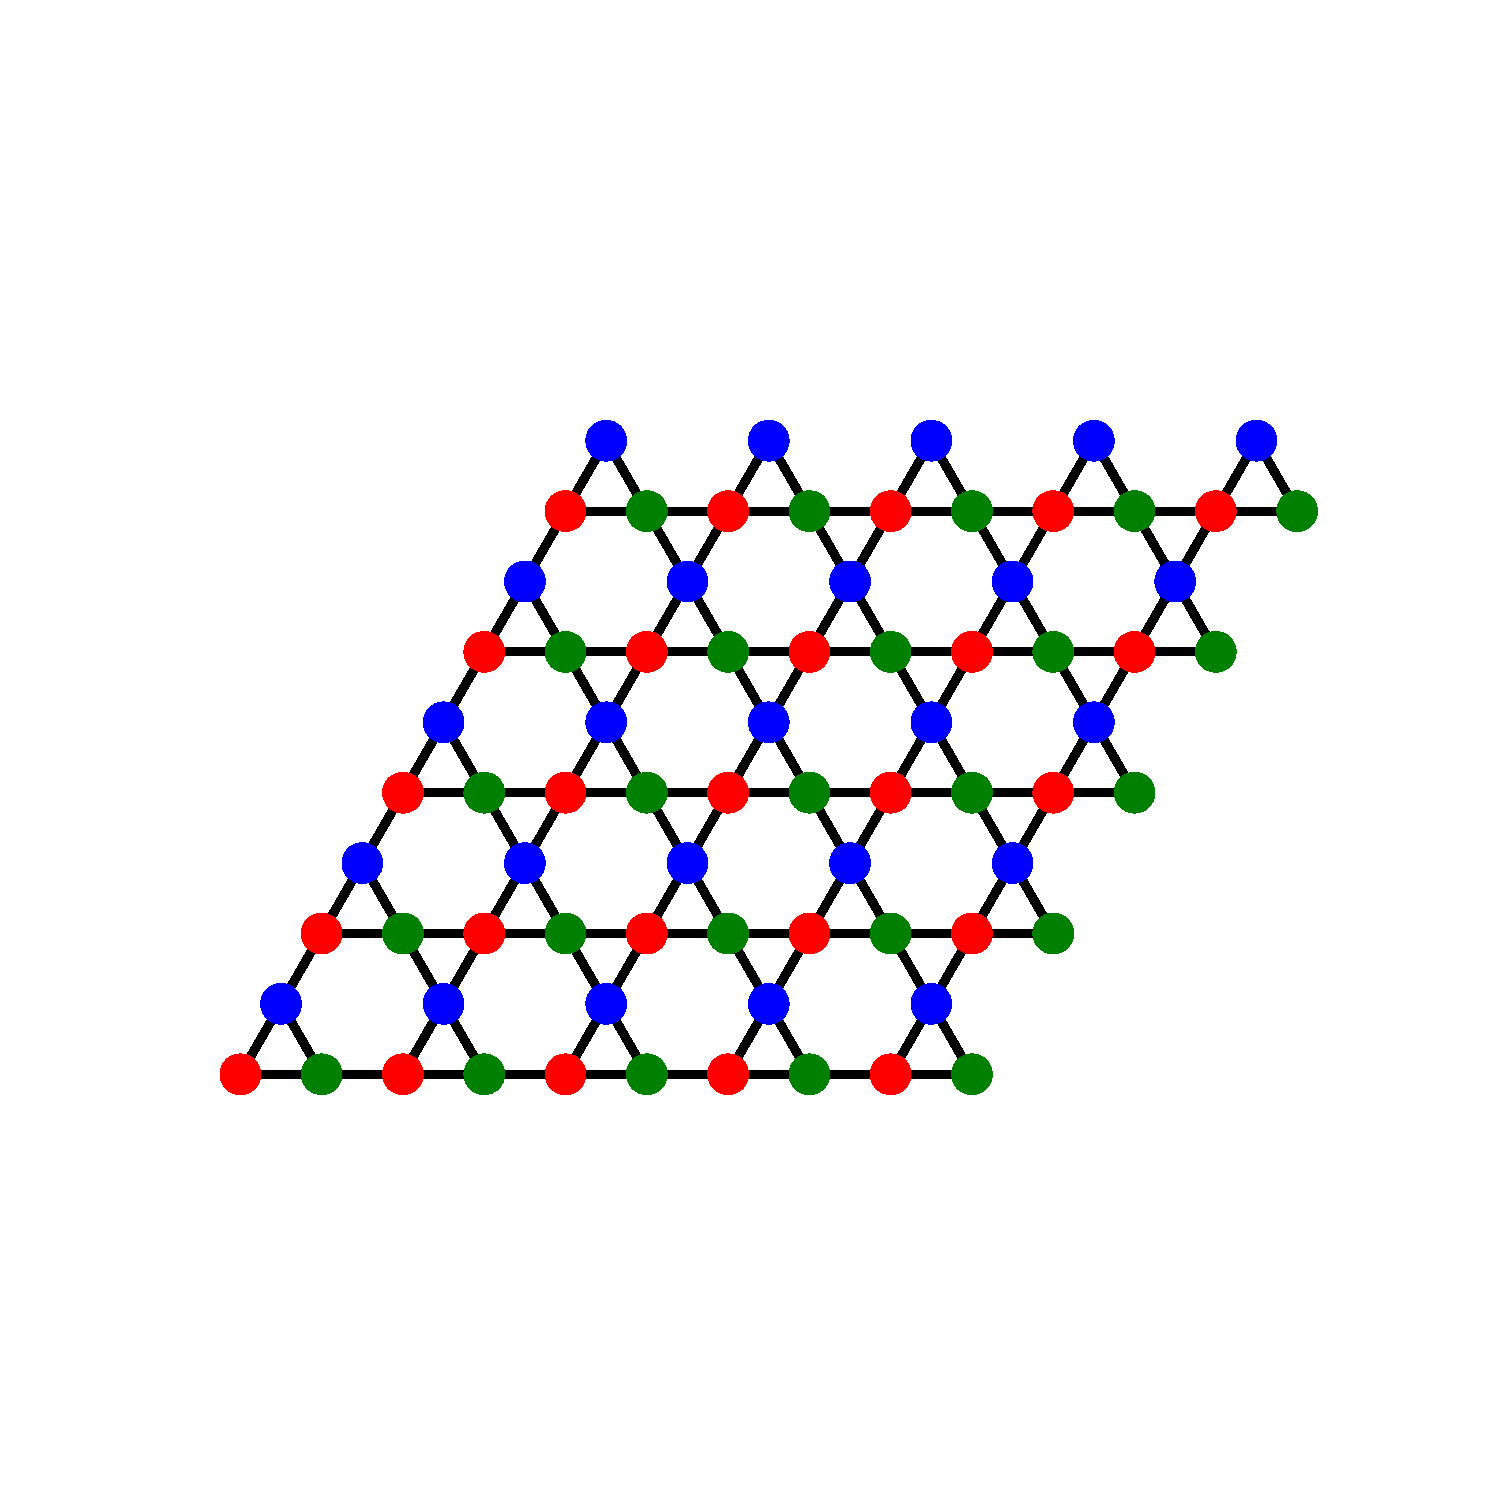
\includegraphics[width=0.49\linewidth]{figs/kagome/lattice.pdf}
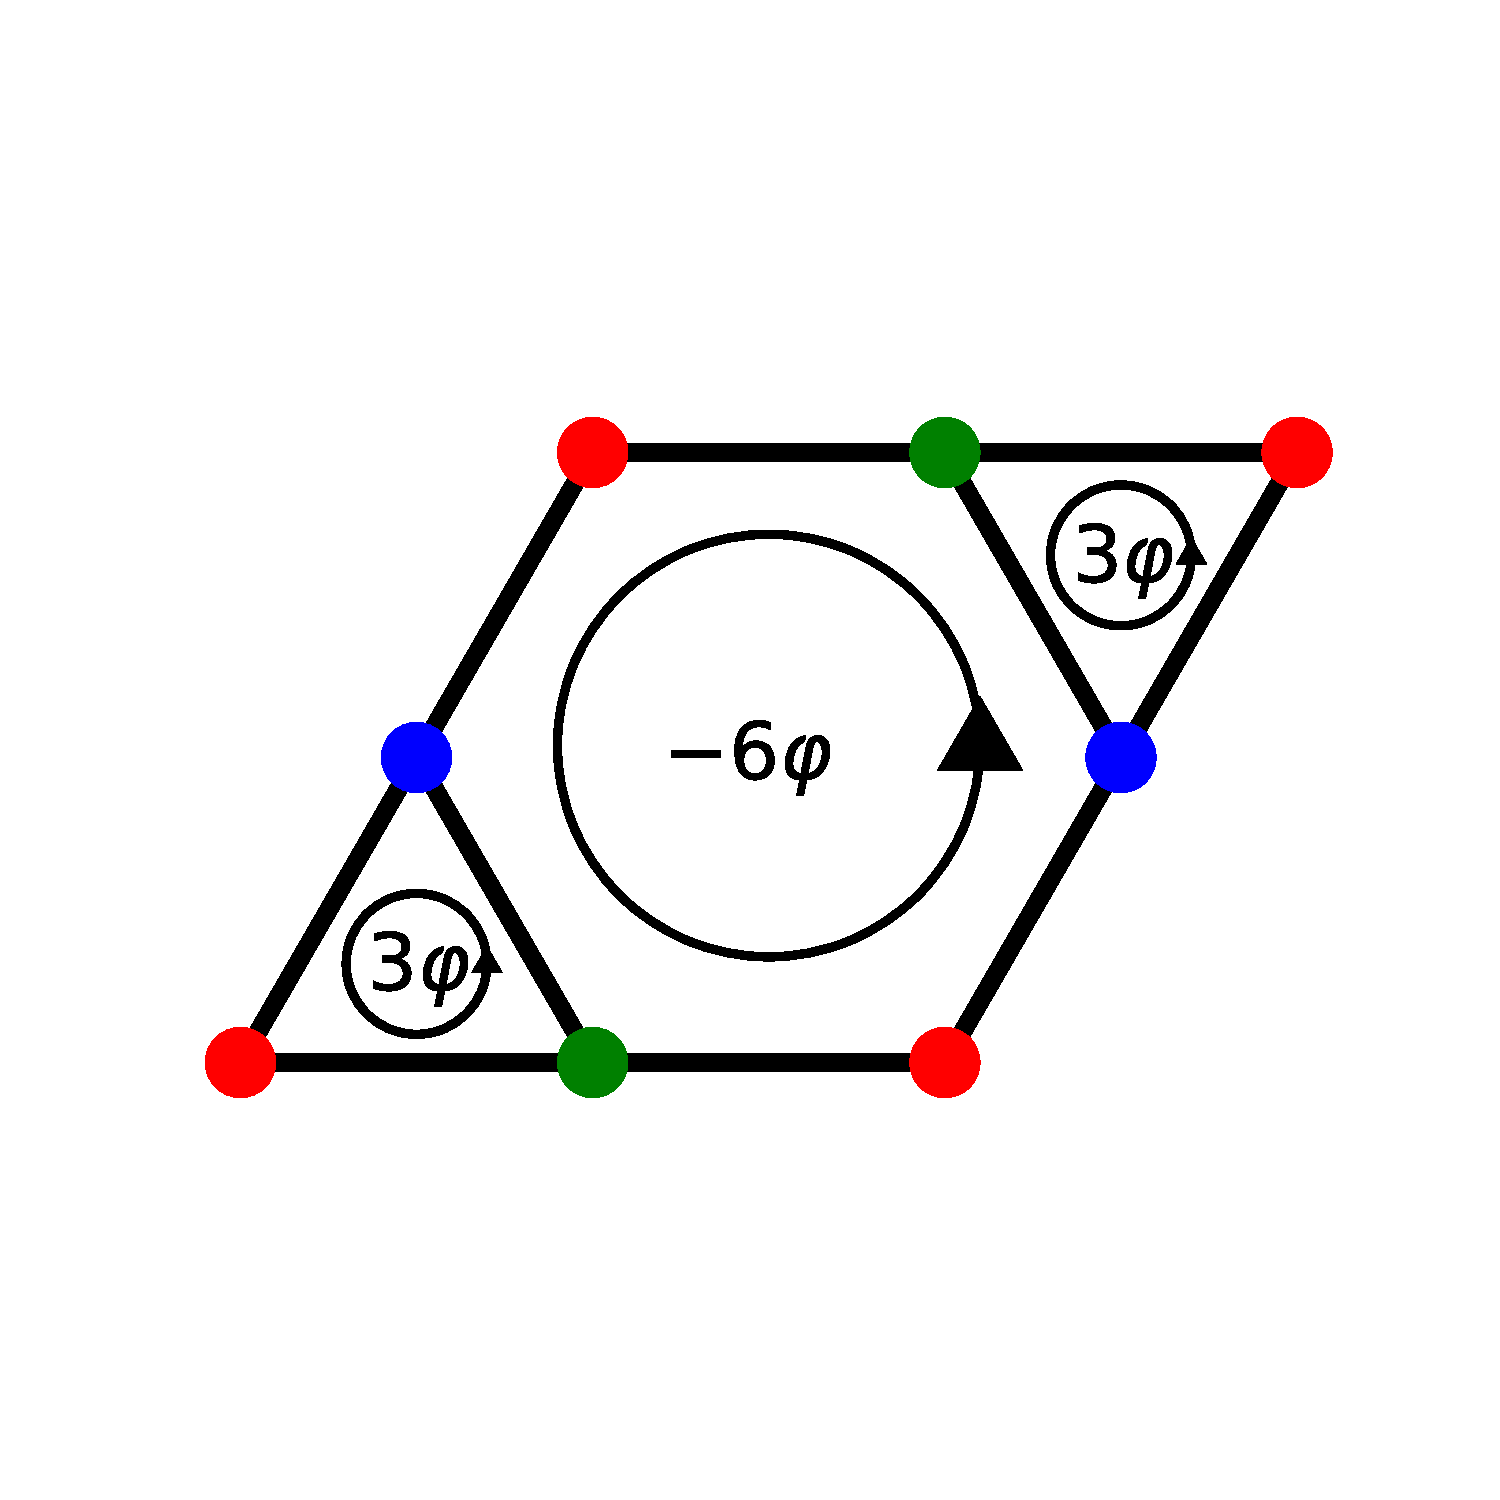
\includegraphics[width=0.49\linewidth]{figs/kagome/flux.pdf}
\begin{picture}(0,0)
{\def\unitlength{}
\put(0.338\linewidth,0.395\linewidth){\line(1,0){17pt}}
\put(0.303\linewidth,0.33\linewidth){\line(1,0){17pt}}
\put(0.303\linewidth,0.33\linewidth){\line(1,2){7pt}}
\put(0.381\linewidth,0.33\linewidth){\line(1,2){7pt}}
\put(0.41\linewidth,0.362\linewidth){\vector(1,0){55pt}}
\put(0.05\linewidth,0.1\linewidth){\small Localized states: $\ket{\mathbf{r}} = \frac{1}{\sqrt{6}} (\sum_{m}(-1)^{m}e^{2im\varphi}a_{\mathbf{r}_{m}}^{\dagger})\ket{0}$}
}
\end{picture}
\end{minipage}
\begin{minipage}{0.15\linewidth}
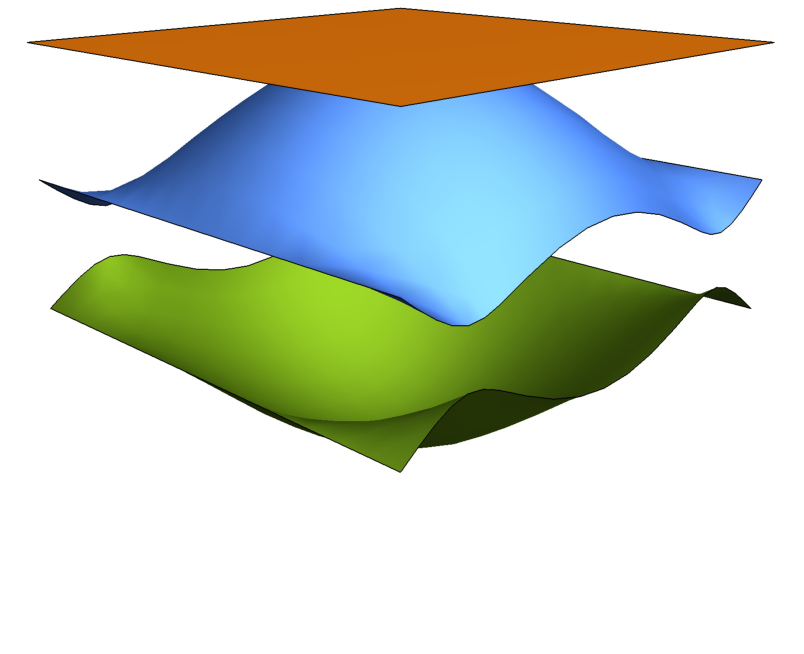
\includegraphics[trim={5 10 5 5},clip,width=\linewidth]{figs/kagome/Pi0.pdf}
\begin{picture}(0,0)
{\def\unitlength{}
\put(0.338\linewidth,0.1\linewidth){\text{$\varphi = 0$}}
}
\end{picture}
\end{minipage}
\begin{minipage}{0.15\linewidth}
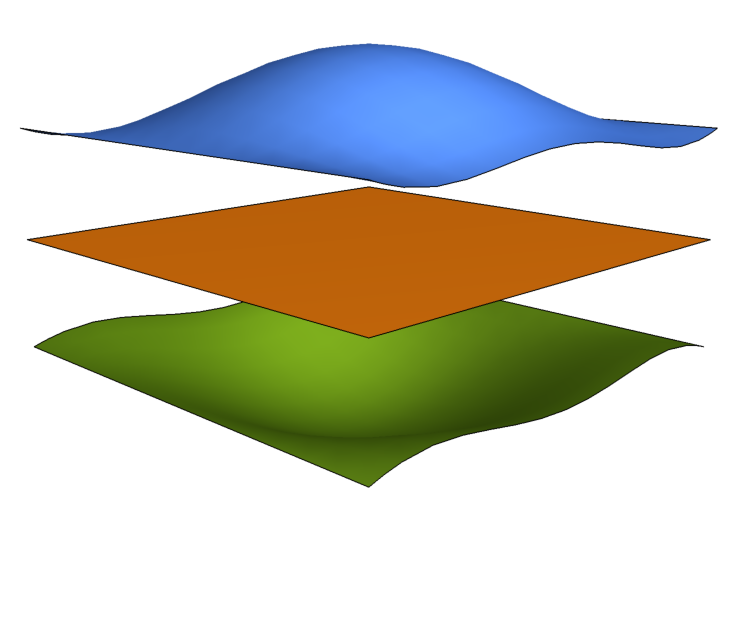
\includegraphics[trim={5 5 5 5},clip,width=\linewidth]{figs/kagome/Pi6.pdf}
\begin{picture}(0,0)
{\def\unitlength{}
\put(0.05\linewidth,0.1\linewidth){\text{$\varphi = \pi/6 \sim \pi/2$}}
}
\end{picture}
\end{minipage}
\begin{minipage}{0.15\linewidth}
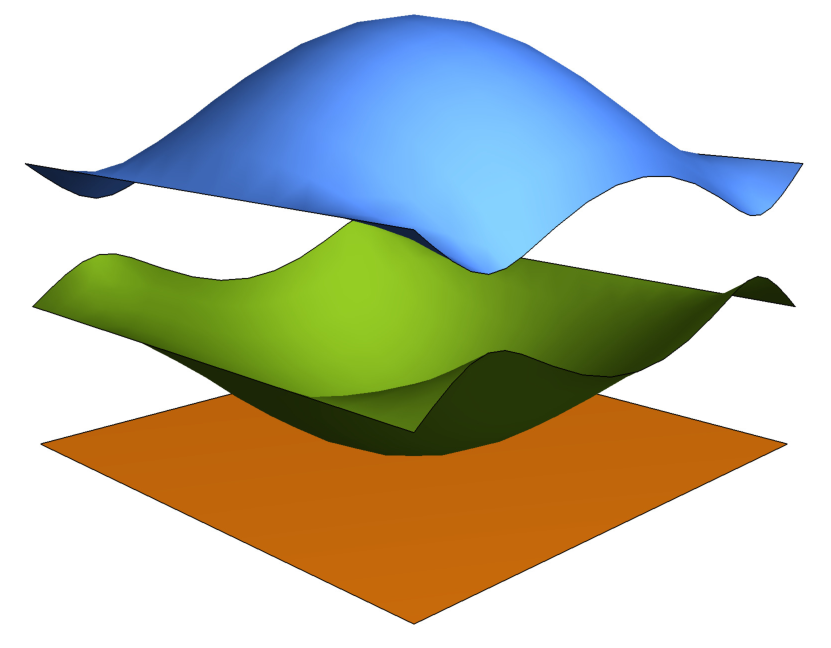
\includegraphics[trim={5 5 5 10},clip,width=\linewidth]{figs/kagome/Pi1.pdf}
\begin{picture}(0,0)
{\def\unitlength{}
\put(0.338\linewidth,0.1\linewidth){\text{$\varphi = \pi$}}
}
\end{picture}
\end{minipage}
\end{figure}


\end{frame}
%----------------------------------------------------------------------------------------
\subsection{Realize SYK model in kagome lattice}
%----------------------------------------------------------------------------------------
\subsubsection{Introducing disorder into flat band}
%----------------------------------------------------------------------------------------
\begin{frame}{Introducing disorder into flat band}
\begin{block}{Impurities on a random subset of lattice sites}
\begin{equation*}
\mathcal{H}_{imp} = u\sum_{i\in R} a_{i}^{\dagger} a_{i}
\end{equation*}
\end{block}

\begin{columns}
\hspace{-3mm}
\begin{column}{0.25\textwidth}
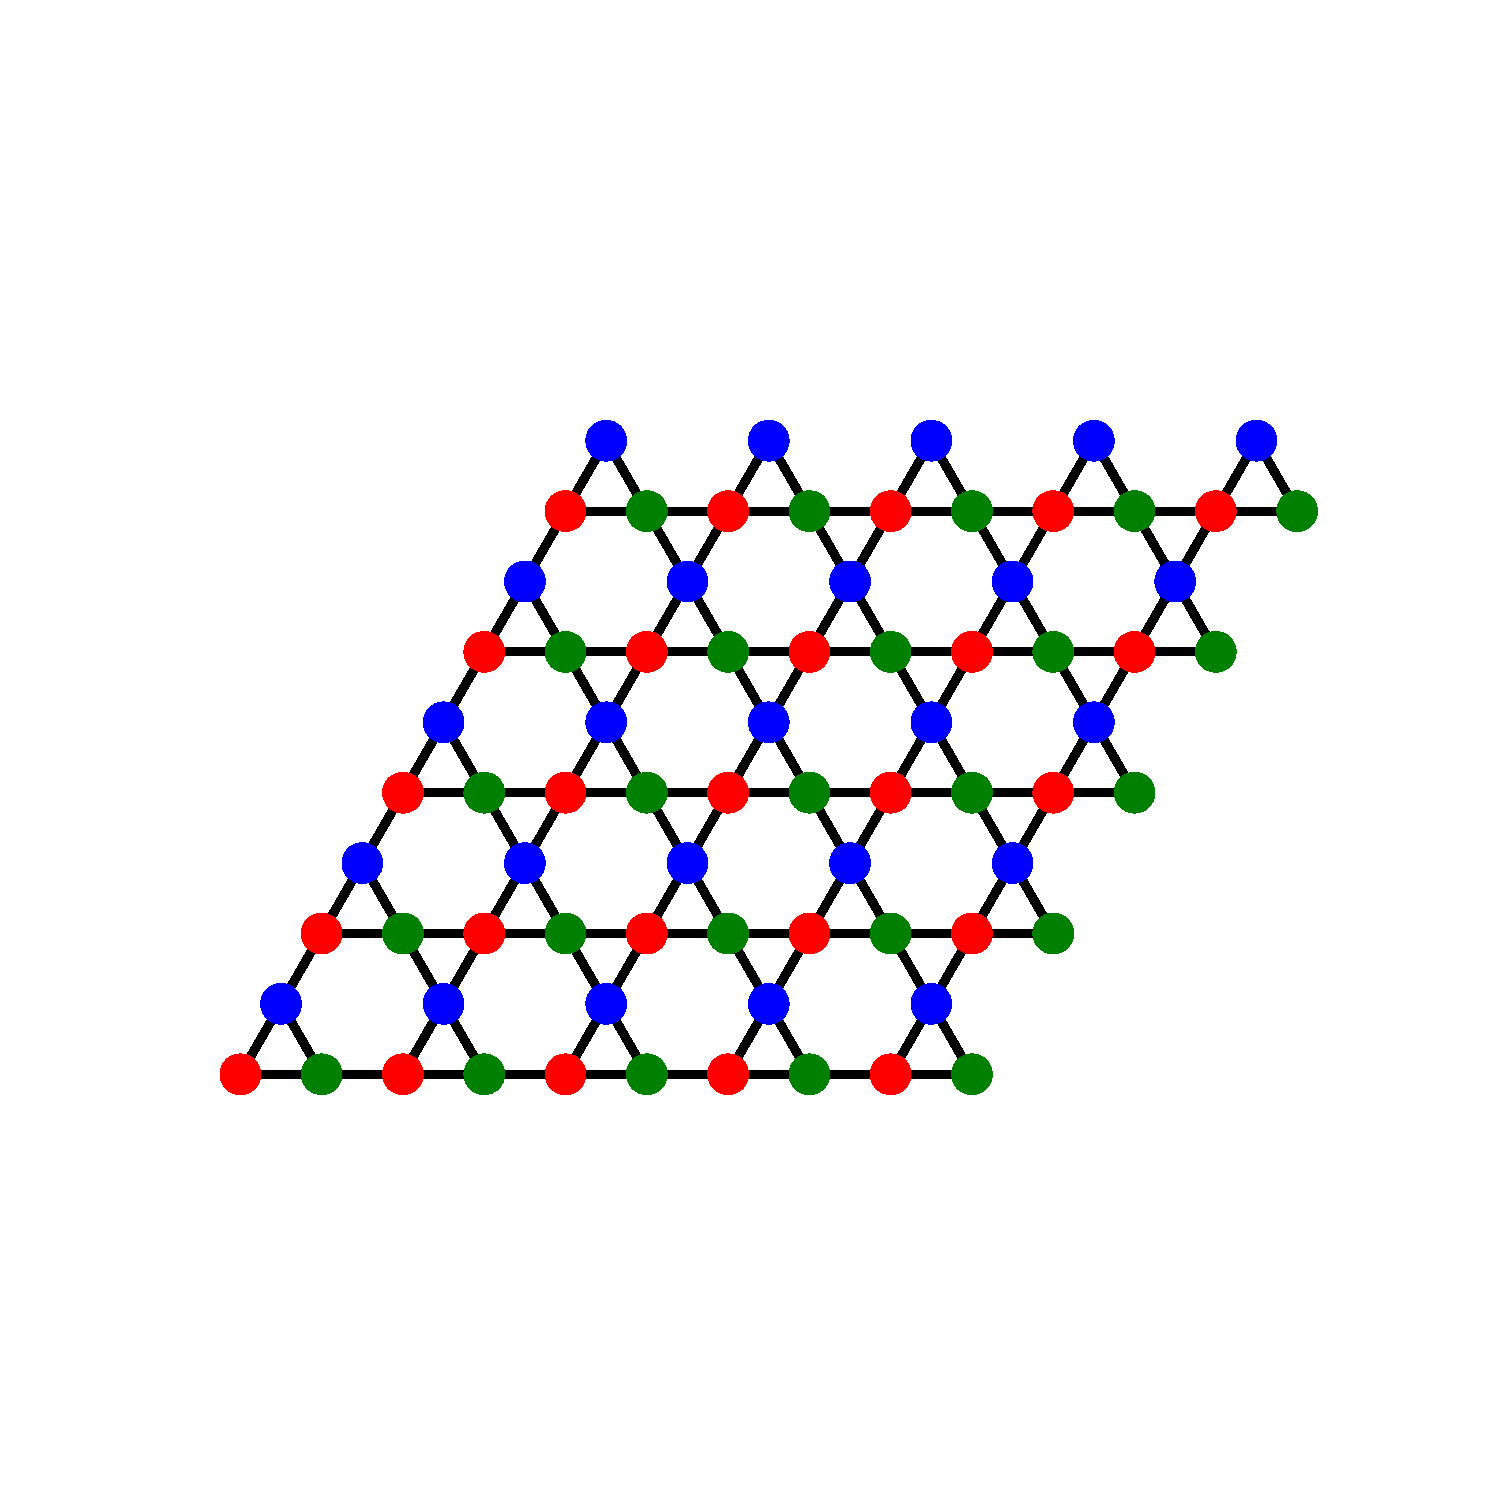
\includegraphics[width=\textwidth]{figs/kagome/lattice.pdf}
\end{column}

\hspace{-3mm}
\begin{column}{0.75\textwidth}
\begin{block}{}
Superposition of co-corner localized states are the eigenstates of $u a_{i}^{\dagger} a_{i}$:

\begin{equation*}
\begin{aligned}
u a_{i}^{\dagger} a_{i} ~ (\ket{\mathbf{r}} + e^{6 i \varphi}\ket{\mathbf{r}'}) &= 0\\
u a_{i}^{\dagger} a_{i} ~ (\ket{\mathbf{r}} - e^{6 i \varphi}\ket{\mathbf{r}'}) &= \frac{2u}{7} (\ket{\mathbf{r}} - e^{6 i \varphi}\ket{\mathbf{r}'})
\end{aligned}
\end{equation*}
\end{block}
\end{column}
\end{columns}
\end{frame}
%----------------------------------------------------------------------------------------
\subsubsection{Effective random interaction}
%----------------------------------------------------------------------------------------
\begin{frame}{Effective random interaction}
\begin{block}{Effective two body interaction Hamiltonian}
\begin{equation*}
\mathcal{H}_{eff} = (2\tilde{t} - \mu) \sum_{i} c_{i}^{\dagger} c_{i} + \sum_{i>j,k>l} J_{ijkl} c_{i}^{\dagger} c_{j}^{\dagger} c_{k} c_{l}
\end{equation*}
\vspace{-3mm}
\begin{equation*}
\begin{aligned}
J_{ijkl} = \frac{1}{2} &\sum_{\mathbf{r}_{1}\mathbf{r}_{2}} [\phi_{i}(\mathbf{r}_{1}) \phi_{j}(\mathbf{r}_{2}) - \phi_{j}(\mathbf{r}_{1}) \phi_{i}(\mathbf{r}_{2})]^{*} \times\\
&V(\mathbf{r}_{1}-\mathbf{r}_{2}) [\phi_{k}(\mathbf{r}_{1}) \phi_{l}(\mathbf{r}_{2}) - \phi_{l}(\mathbf{r}_{1}) \phi_{k}(\mathbf{r}_{2})]
\end{aligned}
\end{equation*}
\end{block}

\begin{figure}
\begin{minipage}{0.24\textwidth}
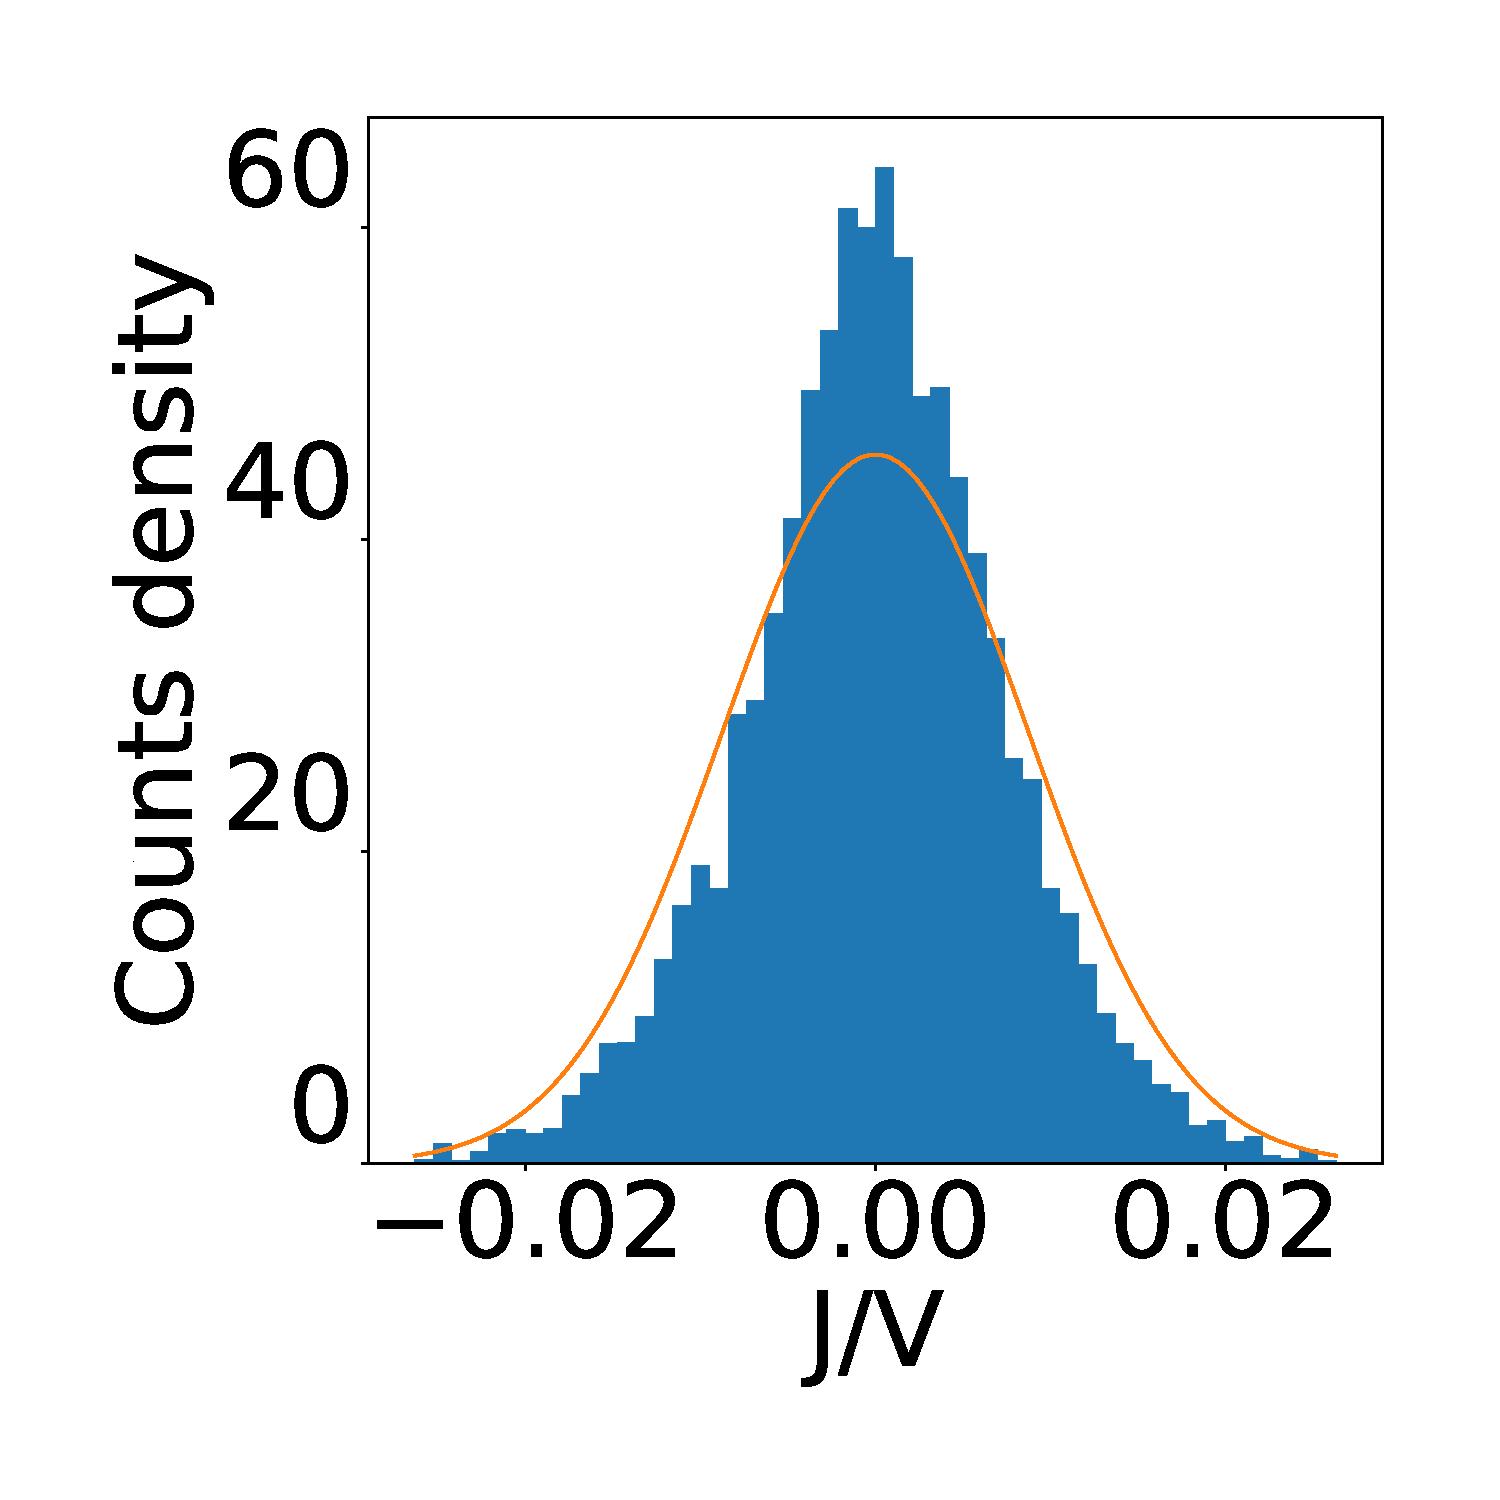
\includegraphics[width=\textwidth]{figs/kagome/1_J_15.pdf}
\begin{picture}(0,0)
{\def\unitlength{}
\put(0.69\linewidth,0.65\linewidth){\text{\tiny Gaussian}}
\put(0.83\linewidth,0.63\linewidth){\vector(-1,-2){8pt}}
}
\end{picture}
\end{minipage}
\begin{minipage}{0.24\textwidth}
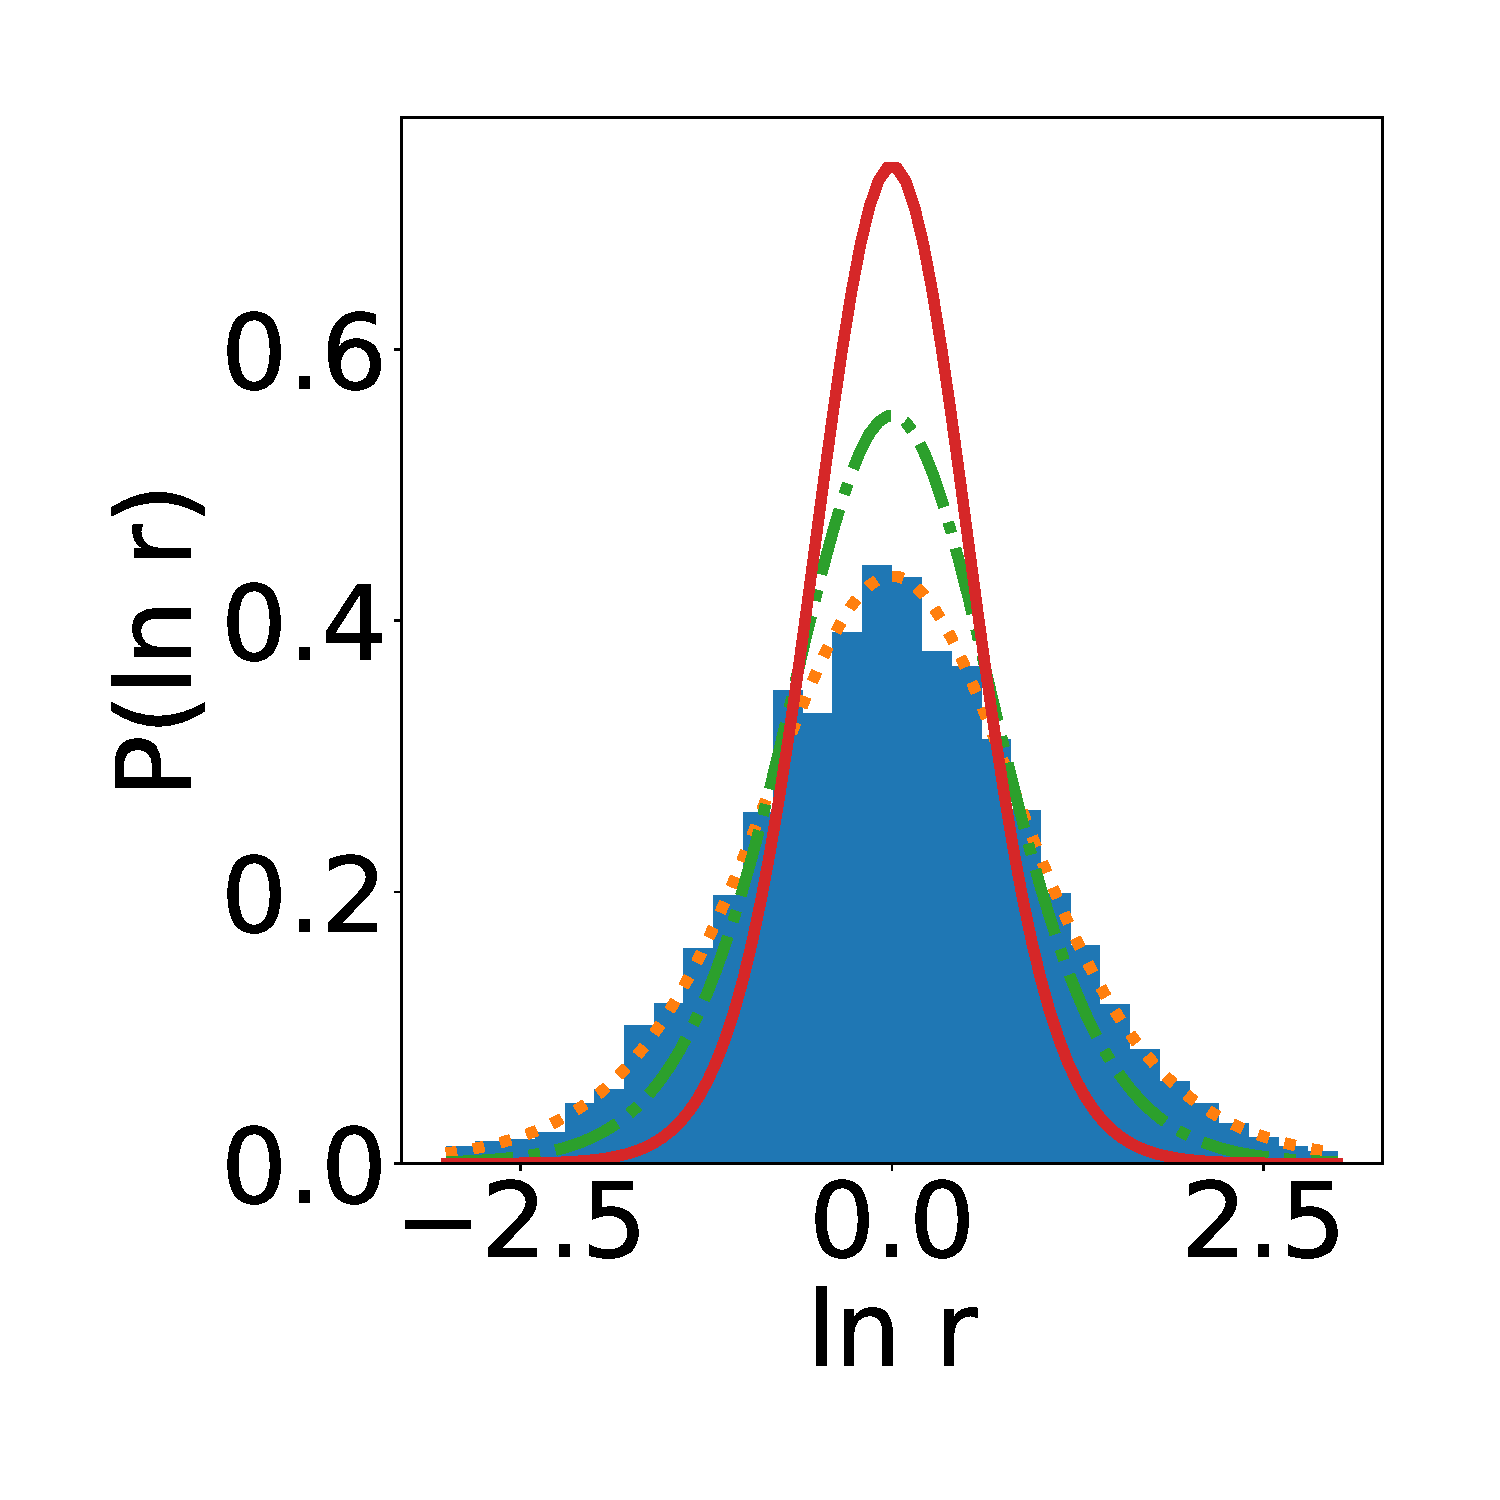
\includegraphics[width=\textwidth]{figs/kagome/1_r_15.pdf}
\begin{picture}(0,0)
{\def\unitlength{}
\put(0.8\linewidth,0.78\linewidth){\text{\tiny GSE}}
\put(0.8\linewidth,0.8\linewidth){\vector(-1,0){16pt}}
\put(0.8\linewidth,0.68\linewidth){\text{\tiny GUE}}
\put(0.8\linewidth,0.7\linewidth){\vector(-1,0){15pt}}
\put(0.8\linewidth,0.58\linewidth){\text{\tiny GOE}}
\put(0.8\linewidth,0.6\linewidth){\vector(-1,0){14pt}}
\put(0.35\linewidth,1.1\linewidth){\text{\tiny $r_{n}=\frac{E_{n+1}-E_{n}}{E_{n}-E_{n-1}}$}}
}
\end{picture}
\end{minipage}
\begin{minipage}{0.24\textwidth}
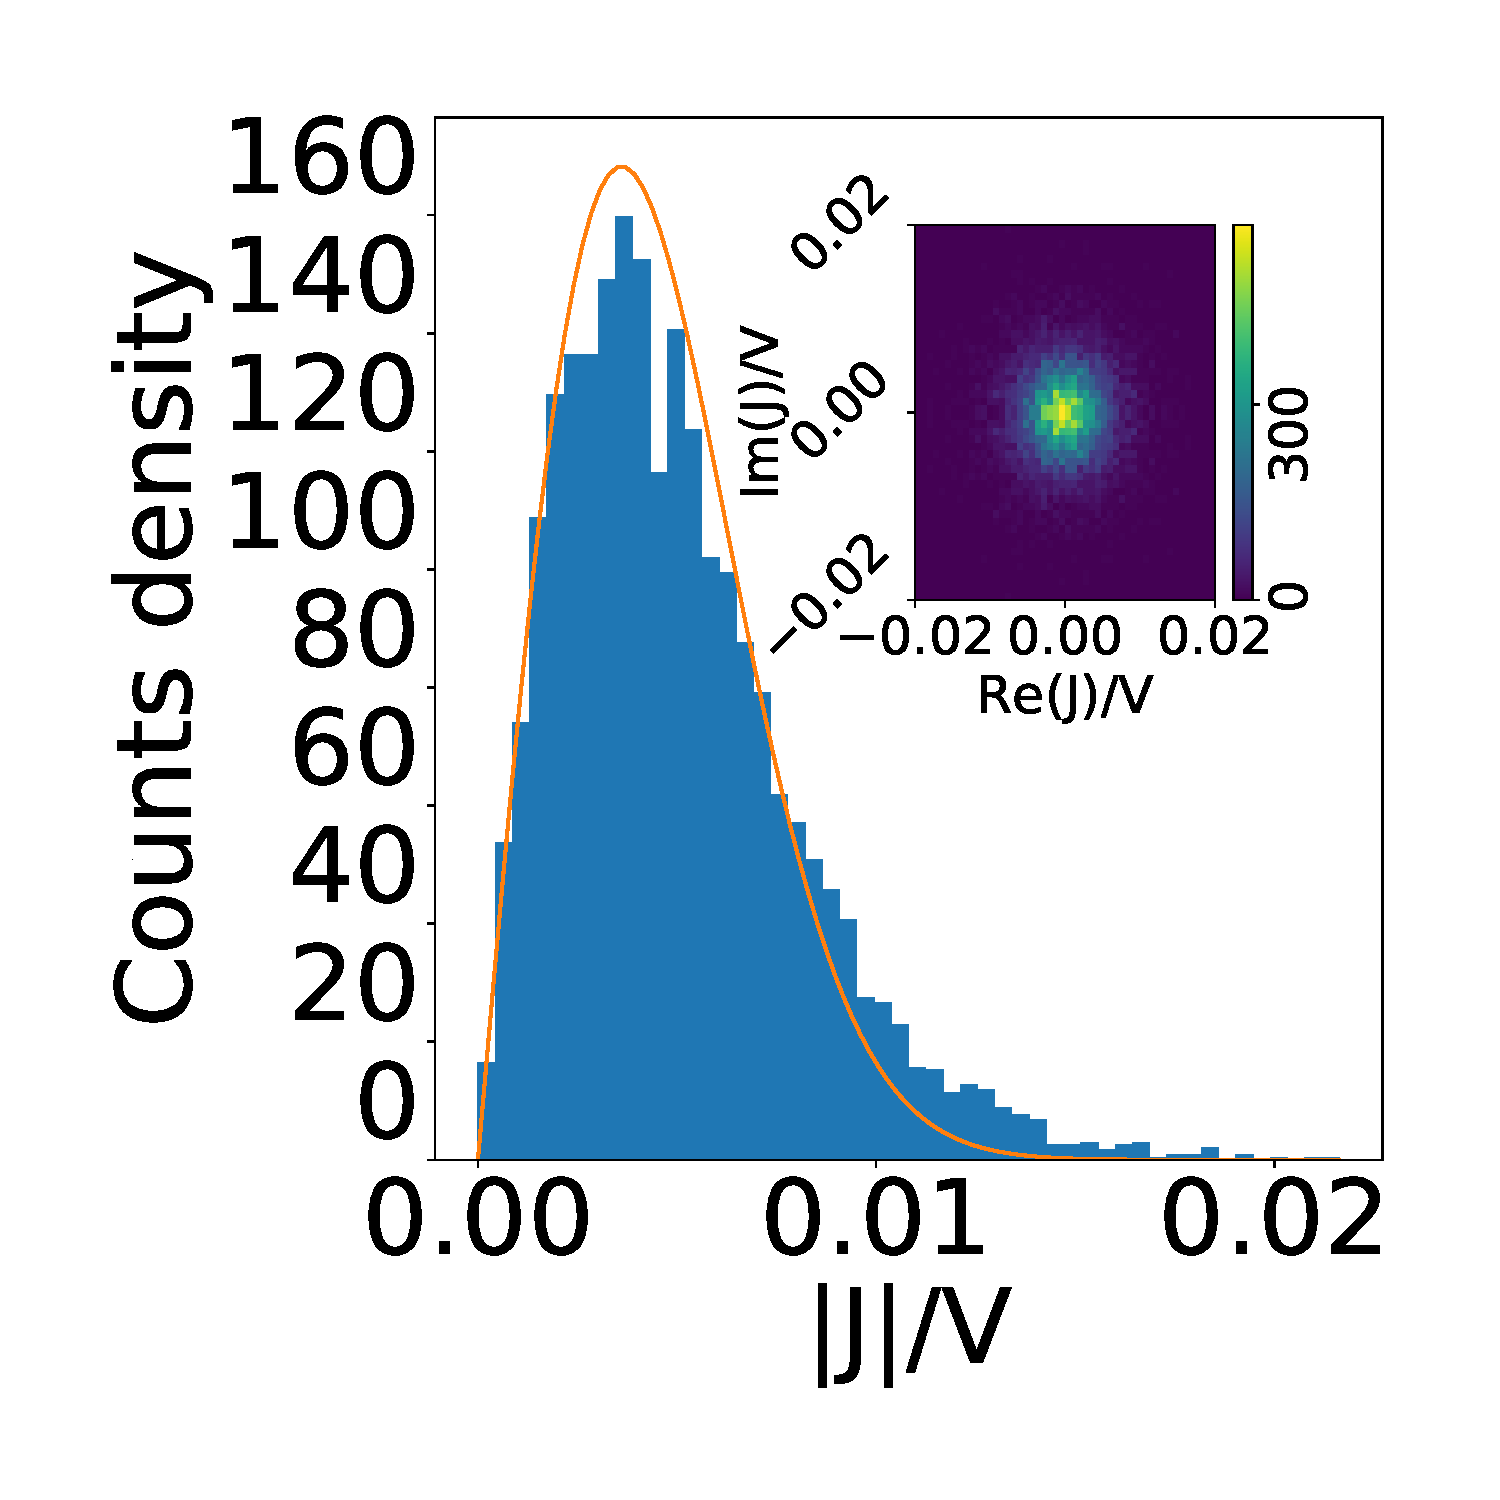
\includegraphics[width=\textwidth]{figs/kagome/T_J_15_insert.pdf}
\begin{picture}(0,0)
{\def\unitlength{}
\put(0.69\linewidth,0.58\linewidth){\text{\tiny Chi}}
\put(0.68\linewidth,0.6\linewidth){\vector(-1,0){17pt}}
}
\end{picture}
\end{minipage}
\begin{minipage}{0.24\textwidth}
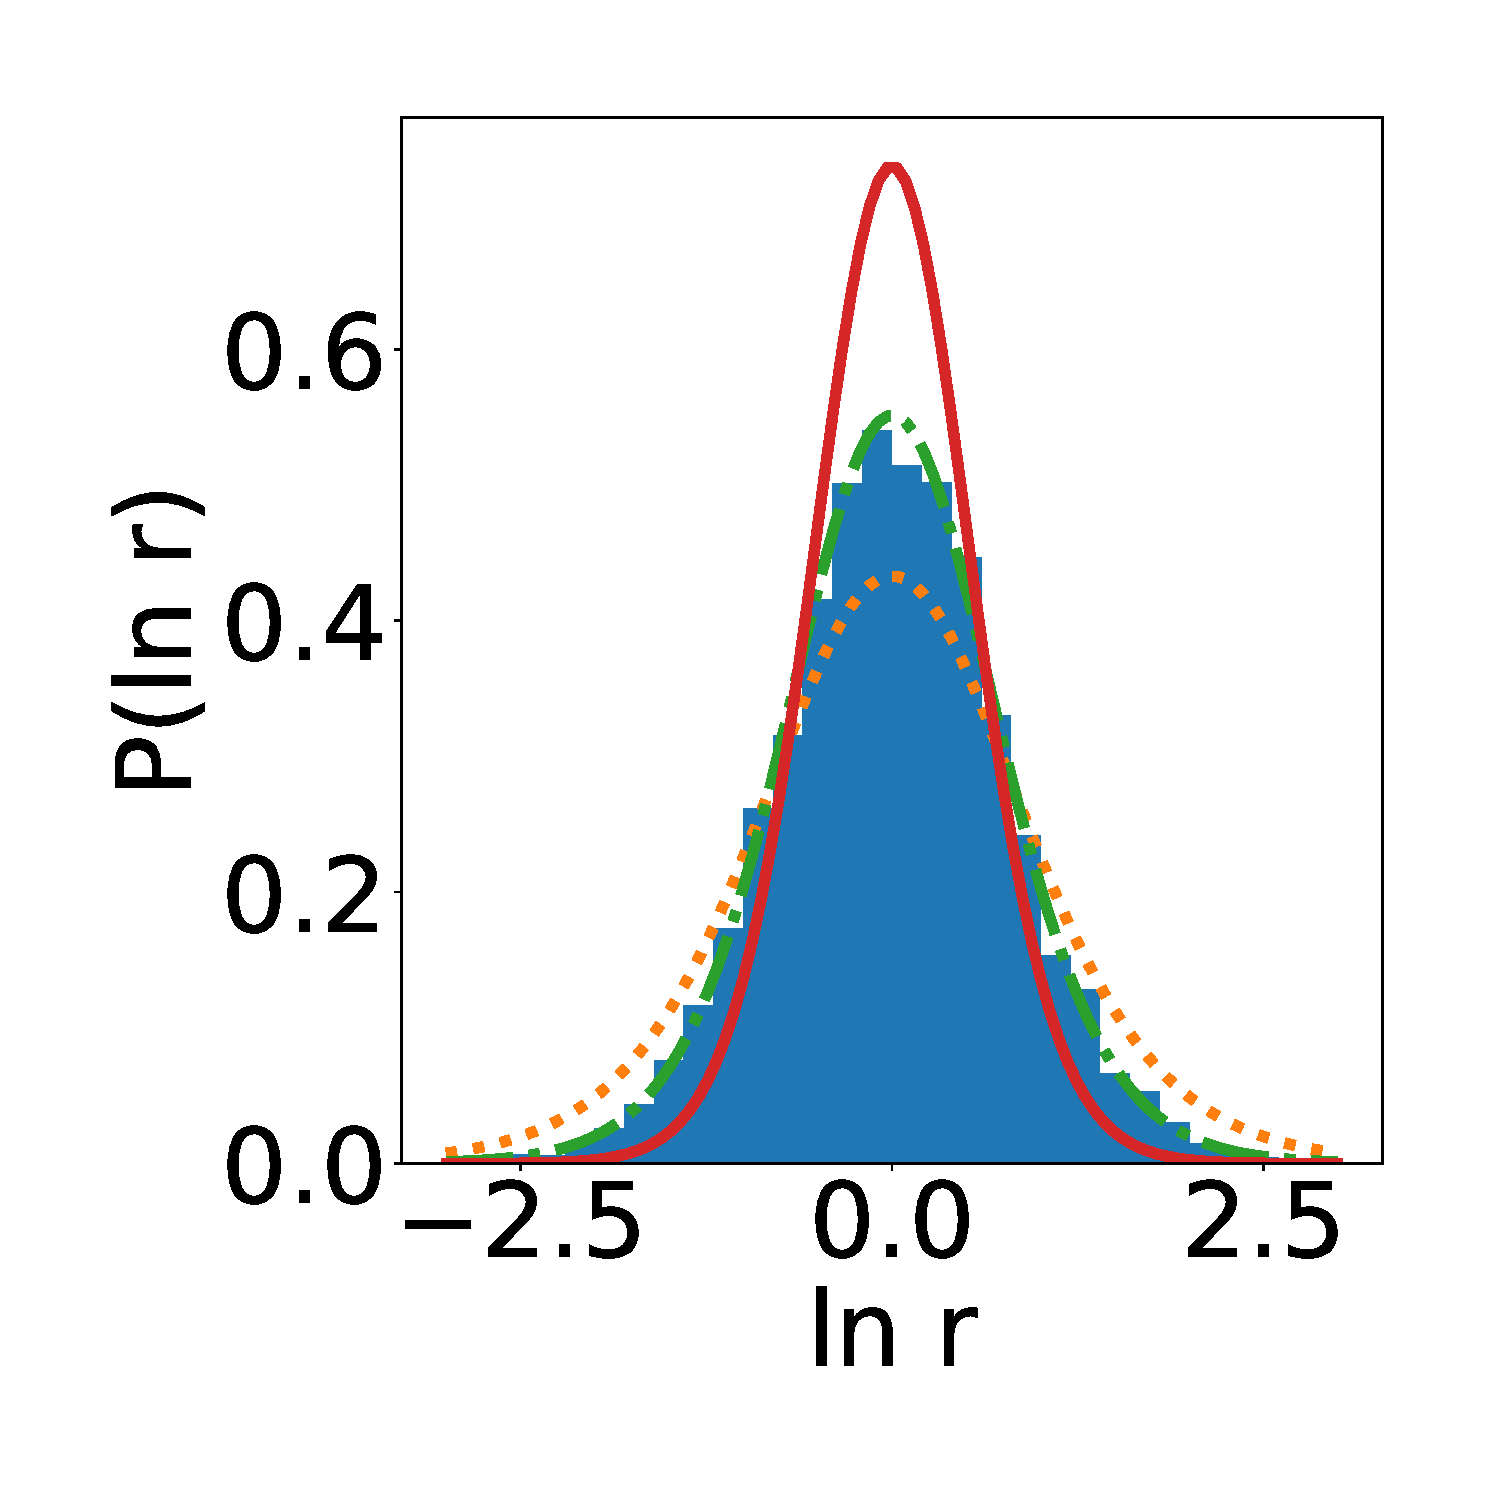
\includegraphics[width=\textwidth]{figs/kagome/T_r_15.pdf}
\begin{picture}(0,0)
{\def\unitlength{}
\put(0.8\linewidth,0.78\linewidth){\text{\tiny GSE}}
\put(0.8\linewidth,0.8\linewidth){\vector(-1,0){16pt}}
\put(0.8\linewidth,0.68\linewidth){\text{\tiny GUE}}
\put(0.8\linewidth,0.7\linewidth){\vector(-1,0){15pt}}
\put(0.8\linewidth,0.58\linewidth){\text{\tiny GOE}}
\put(0.8\linewidth,0.6\linewidth){\vector(-1,0){14pt}}
\put(0.35\linewidth,1.1\linewidth){\text{\tiny $r_{n}=\frac{E_{n+1}-E_{n}}{E_{n}-E_{n-1}}$}}
}
\end{picture}
\end{minipage}
\end{figure}
\end{frame}
%----------------------------------------------------------------------------------------
\subsubsection{Experimental aspects}
%----------------------------------------------------------------------------------------
\begin{frame}{Experimental aspects}

\begin{itemize}
\item Kagome lattice is realized in cold atom systems\footnote[frame]{\cite{jo2012ultracold}}
\vspace{3 mm}

\item Positive or complex hopping\footnote[frame]{\cite{aidelsburger2011experimental,struck2012tunable}}\\
\vspace{3 mm} $\Rightarrow$ artificial gauge fields
$\left\lbrace\parbox{8cm}{
Apply zero averaged homogeneous inertial force\\
Raman-assisted tunneling in asymmetric lattice
}\right.$
\vspace{8 mm}
\item The randomly distributed on-site potential
$\Rightarrow$ Load a mixture of heavy and light atoms
\vspace{8 mm}
\item $J \propto a_p^{3}$ $\Rightarrow$ Feshbach resonances can be used to tune $J$
\end{itemize}

\end{frame}
%----------------------------------------------------------------------------------------
% \subsection{Experimental observables}
%----------------------------------------------------------------------------------------
\subsubsection{Entropy}
%----------------------------------------------------------------------------------------
\subsubsection{Spectral form factor}
%----------------------------------------------------------------------------------------
\subsubsection{Velocity distribution when releasing the optical lattice}
%----------------------------------------------------------------------------------------
\begin{frame}{Experimental observables}
\vspace{-6.5mm}
\begin{figure}
\begin{minipage}{0.24\textwidth}
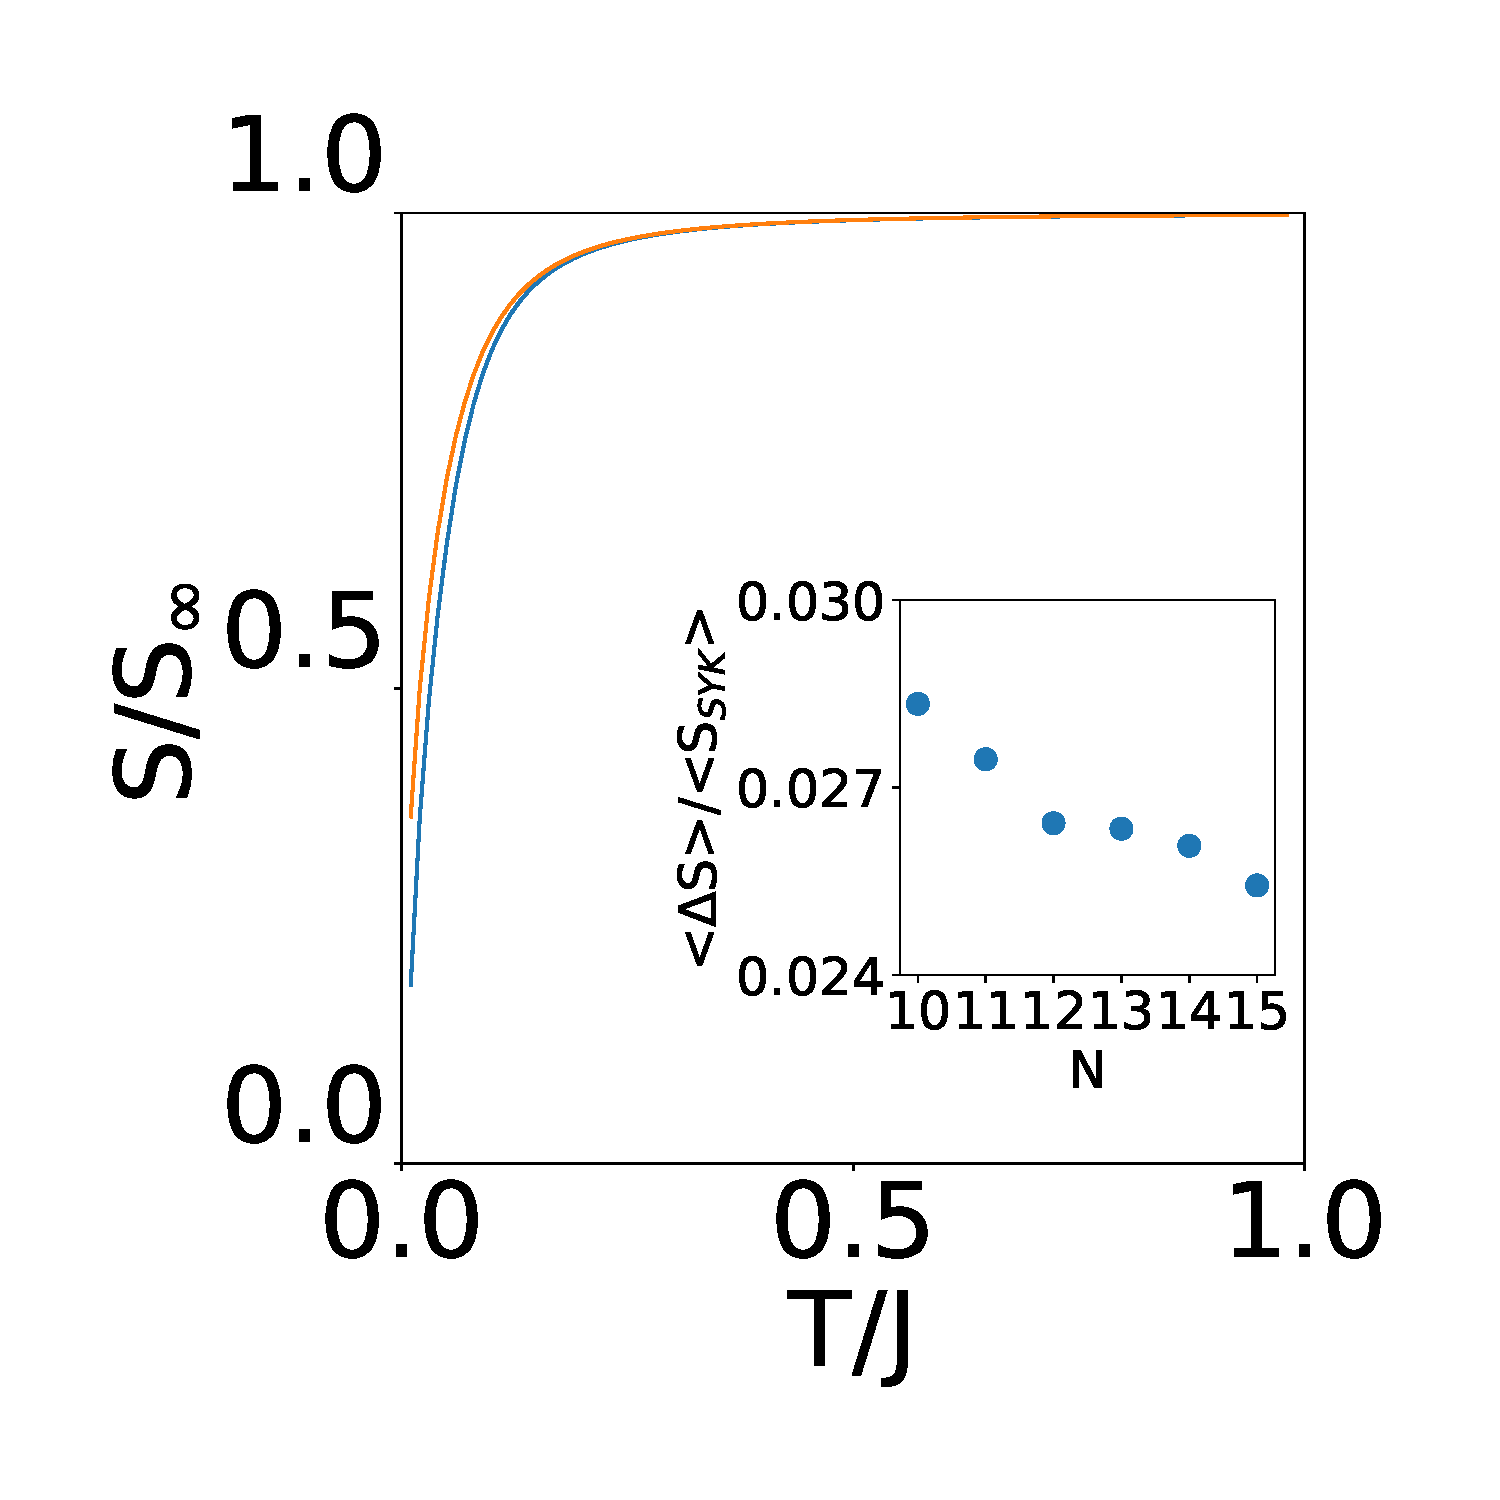
\includegraphics[width=\textwidth]{figs/kagome/T_S_15.pdf}
\begin{picture}(0,0)
{\def\unitlength{}
\put(0.48\linewidth,0.93\linewidth){\text{\tiny Orange: SYK}}
\put(0.38\linewidth,0.88\linewidth){\tiny Blue: ED of $\mathcal{H}_{\mathrm{eff}}$}
}
\end{picture}
\end{minipage}
\begin{minipage}{0.24\textwidth}
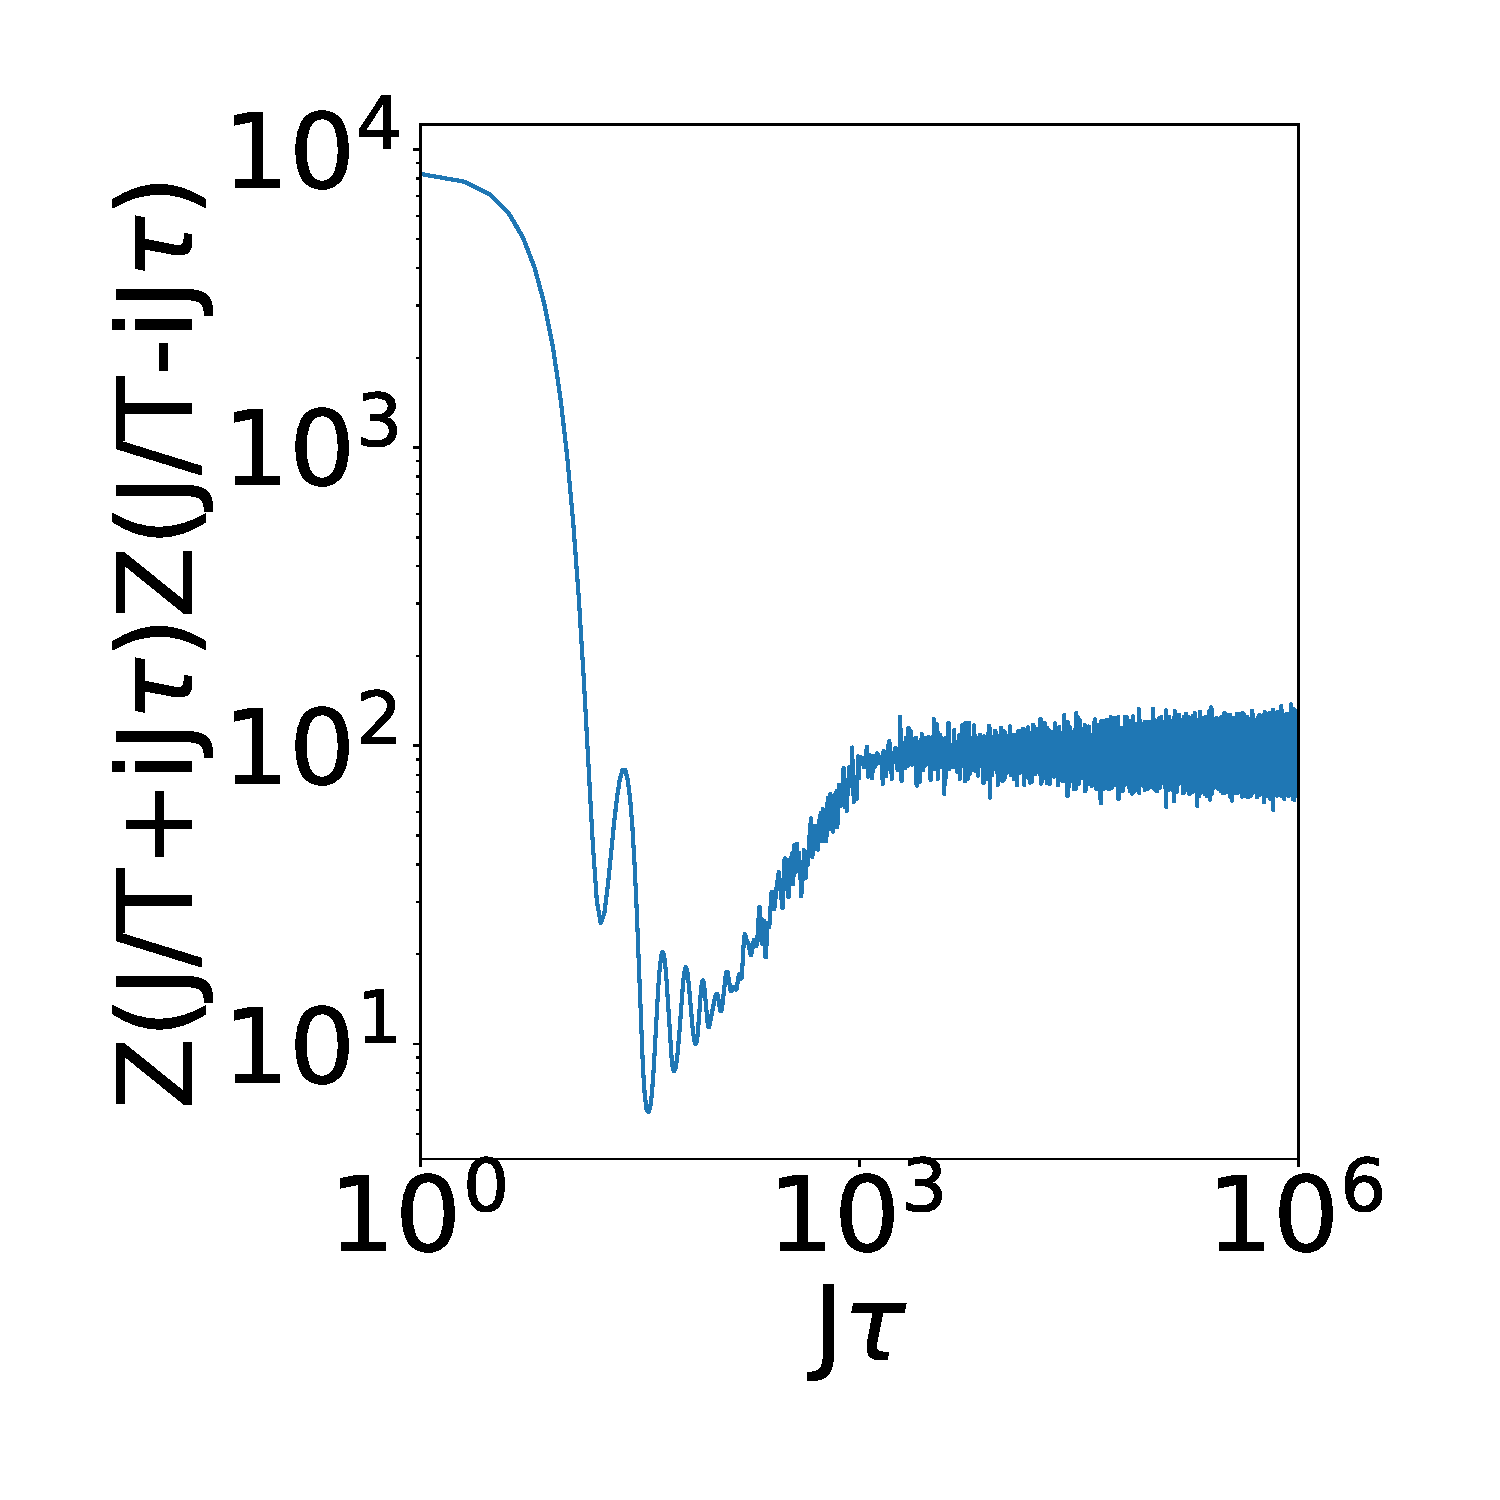
\includegraphics[width=\textwidth]{figs/kagome/T_Z2_14_1.pdf}
\end{minipage}
\begin{minipage}{0.24\textwidth}
\vspace{5mm}
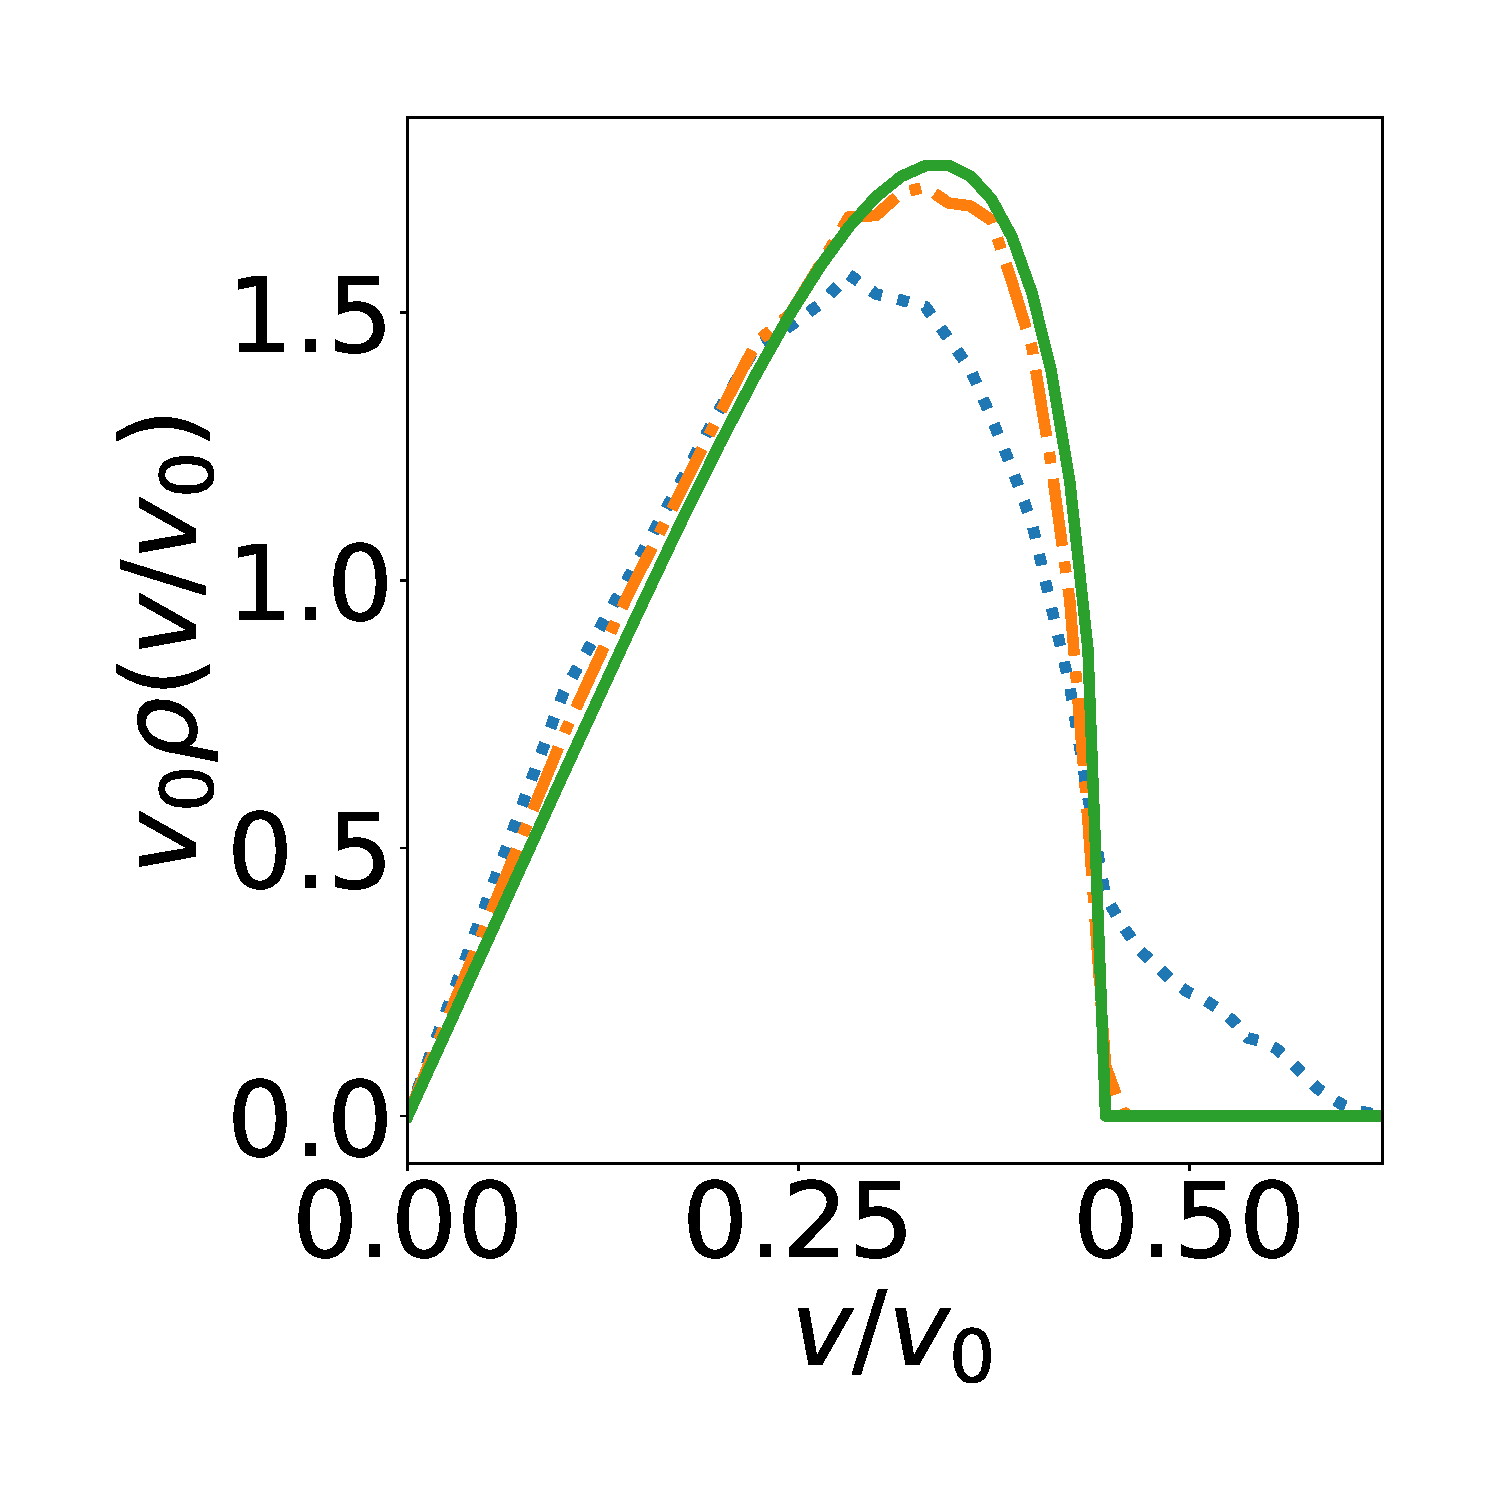
\includegraphics[width=\textwidth]{figs/kagome/T_14_vDis.pdf}
\begin{picture}(0,0)
{\def\unitlength{}
\put(0.275\linewidth,0.52\linewidth){\text{\tiny Green: Wigner semicircle}}
\put(0.275\linewidth,0.45\linewidth){\text{\tiny Orange: SYK}}
\put(0.275\linewidth,0.38\linewidth){\tiny$\text{Blue: ED of }\mathcal{H}_{\mathrm{eff}}$}
}
\end{picture}
\end{minipage}
\begin{minipage}{0.24\textwidth}
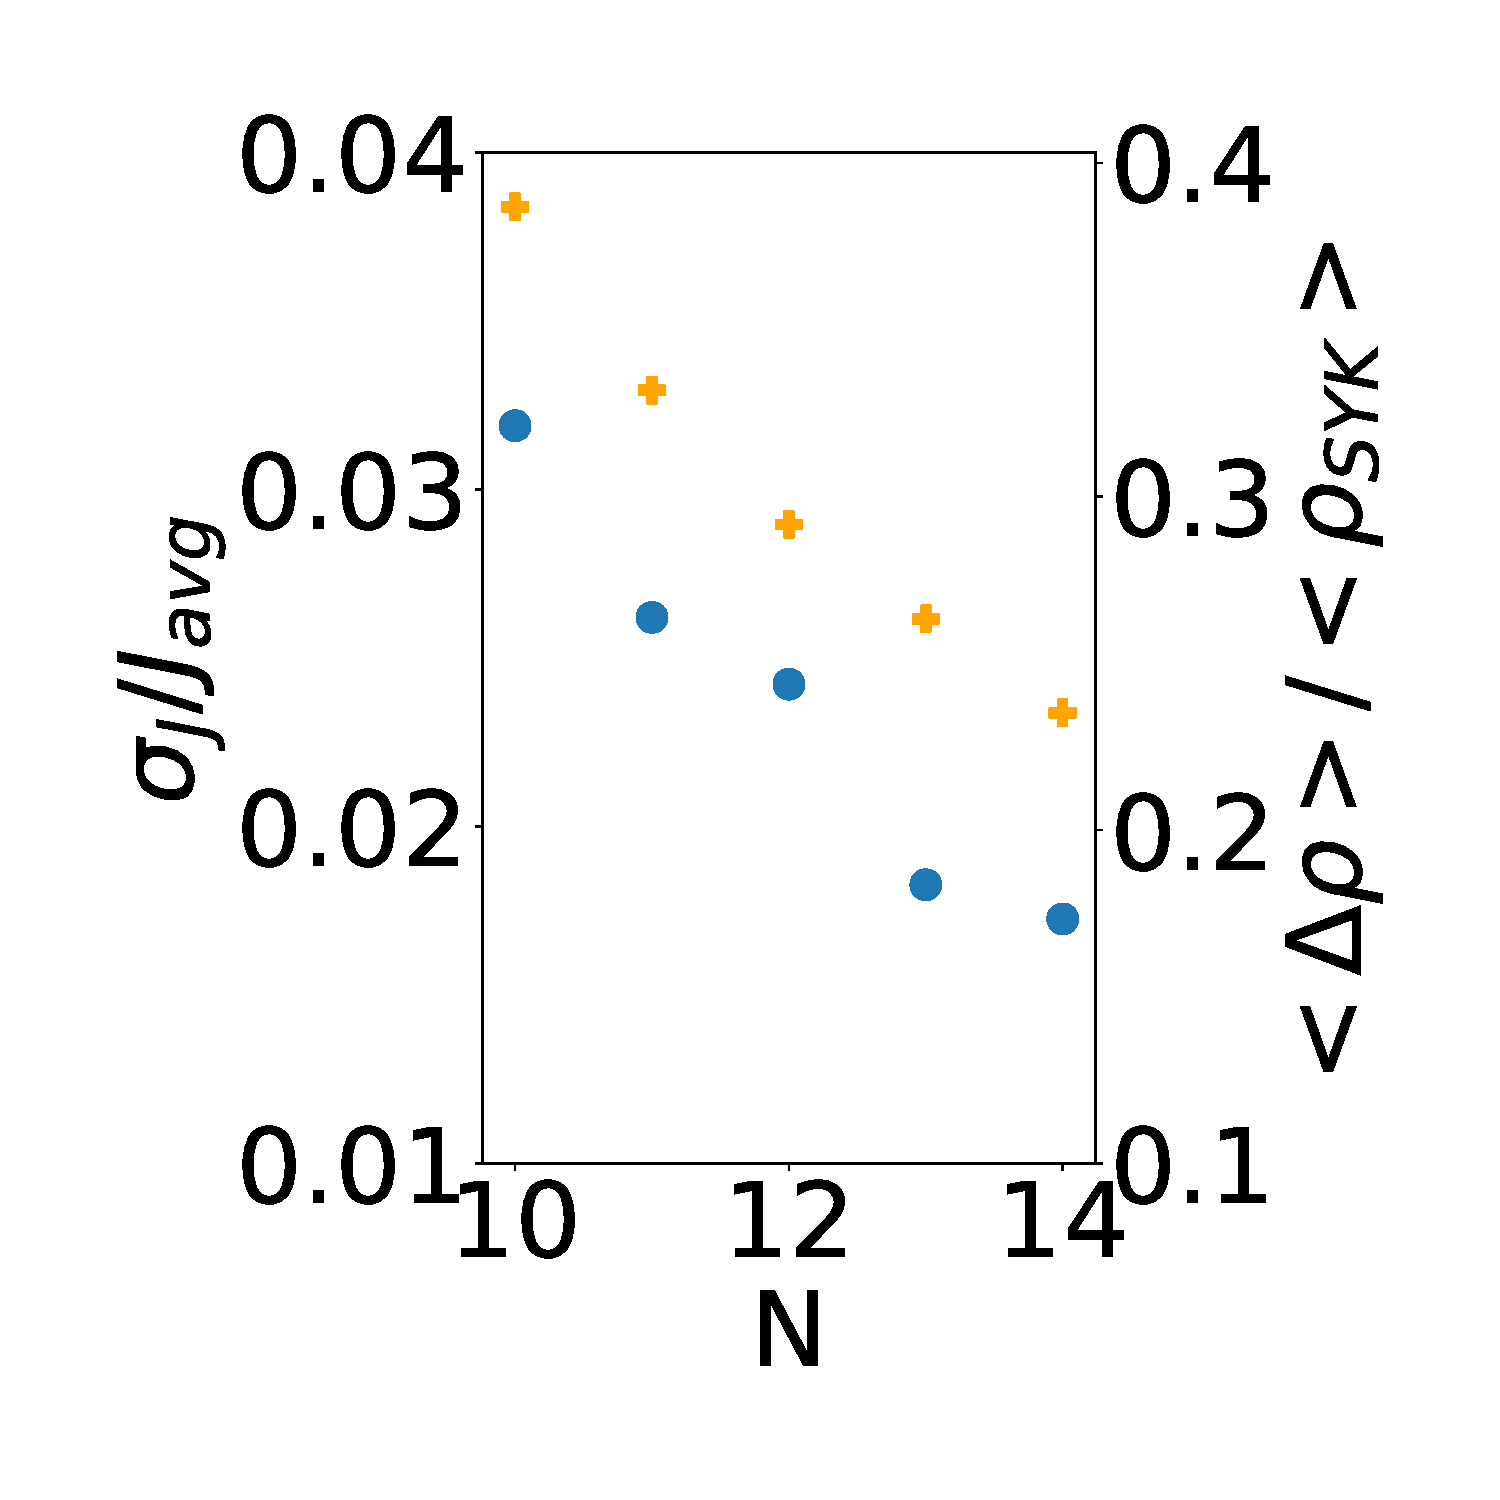
\includegraphics[width=\textwidth]{figs/kagome/DJ0.pdf}
\end{minipage}
\end{figure}

\vspace{-8.5mm}

\begin{itemize}
\item The zero temperature entropy will be a finite number as $N \to \infty$.

\item $\frac{1}{N} \sum_i \langle c_{i}(0) c_{i}^{\dagger}(\tau) \rangle \propto Z(\beta J+iJ\tau)Z(\beta J-iJ\tau)$(spectral form factor)\footnote[frame]{\cite{cotler2017chaos,saad2019semiclassical}}:
\subitem{For $\tau\to0$, $|Z(\beta J+iJ\tau)|^{2}\propto\tau^{-\alpha}$(no quasi-particles).}
\subitem{For $\tau\to\infty$, $|Z(\beta J+iJ\tau)|^{2}=Z(2\beta J)$.}
\subitem{For intermediate $\tau$, $|Z(\beta J+iJ\tau)|^{2}\propto\tau$(random matrix theory).}

\item Velocity distribution will show a decay tail.
\end{itemize}

\end{frame}

%----------------------------------------------------------------------------------------
% \begin{frame}{Other proposals\footnote[frame]{\cite{franz2018mimicking}}}
% \begin{columns}
% \begin{column}{0.5\textwidth}
% \begin{figure}
% \begin{minipage}{\textwidth}
% 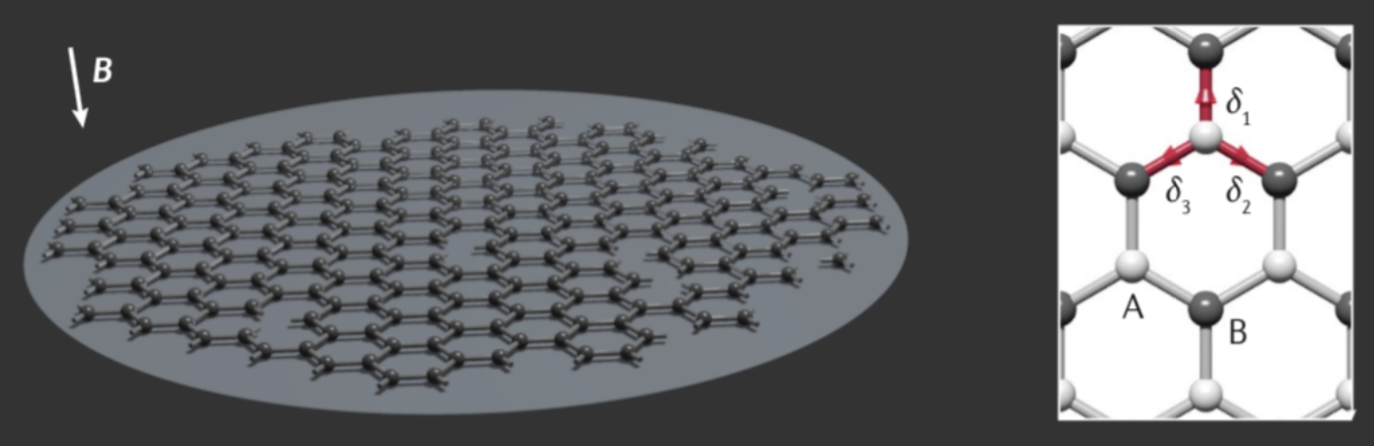
\includegraphics[width=\textwidth]{figs/SYK/r1.png}
% \end{minipage}
% \begin{minipage}{\textwidth}
% 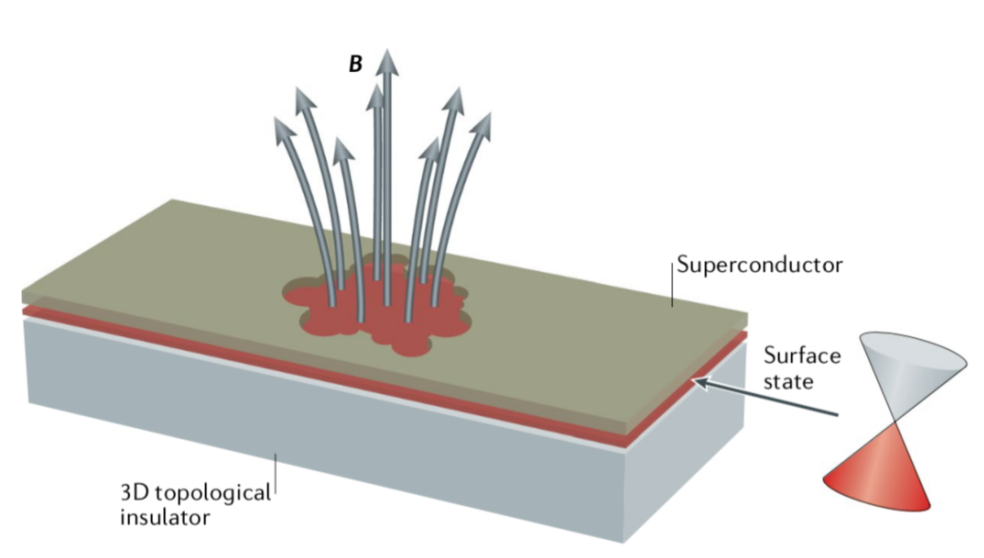
\includegraphics[width=\textwidth]{figs/SYK/r2.png}
% \end{minipage}
% \end{figure}
% \end{column}
% \begin{column}{0.5\textwidth}
% Graphene flake in a strong magnetic field with irregular boundary

% \vspace{3cm}
% Fu-Kane superconductor with irregular-shaped holes
% \end{column}
% \end{columns}
% \end{frame}